\documentclass[10pt]{article}
% TMLR official style (github.com/JmlrOrg/tmlr-style-file, fetched 2026-10-05), anonymous submission mode
% (no [accepted] / [preprint] option).
\usepackage{tmlr}
%%%%% NEW MATH DEFINITIONS %%%%%

\usepackage{amsmath,amsfonts,bm}

% Mark sections of captions for referring to divisions of figures
\newcommand{\figleft}{{\em (Left)}}
\newcommand{\figcenter}{{\em (Center)}}
\newcommand{\figright}{{\em (Right)}}
\newcommand{\figtop}{{\em (Top)}}
\newcommand{\figbottom}{{\em (Bottom)}}
\newcommand{\captiona}{{\em (a)}}
\newcommand{\captionb}{{\em (b)}}
\newcommand{\captionc}{{\em (c)}}
\newcommand{\captiond}{{\em (d)}}

% Highlight a newly defined term
\newcommand{\newterm}[1]{{\bf #1}}


% Figure reference, lower-case.
\def\figref#1{figure~\ref{#1}}
% Figure reference, capital. For start of sentence
\def\Figref#1{Figure~\ref{#1}}
\def\twofigref#1#2{figures \ref{#1} and \ref{#2}}
\def\quadfigref#1#2#3#4{figures \ref{#1}, \ref{#2}, \ref{#3} and \ref{#4}}
% Section reference, lower-case.
\def\secref#1{section~\ref{#1}}
% Section reference, capital.
\def\Secref#1{Section~\ref{#1}}
% Reference to two sections.
\def\twosecrefs#1#2{sections \ref{#1} and \ref{#2}}
% Reference to three sections.
\def\secrefs#1#2#3{sections \ref{#1}, \ref{#2} and \ref{#3}}
% Reference to an equation, lower-case.
\def\eqref#1{equation~\ref{#1}}
% Reference to an equation, upper case
\def\Eqref#1{Equation~\ref{#1}}
% A raw reference to an equation---avoid using if possible
\def\plaineqref#1{\ref{#1}}
% Reference to a chapter, lower-case.
\def\chapref#1{chapter~\ref{#1}}
% Reference to an equation, upper case.
\def\Chapref#1{Chapter~\ref{#1}}
% Reference to a range of chapters
\def\rangechapref#1#2{chapters\ref{#1}--\ref{#2}}
% Reference to an algorithm, lower-case.
\def\algref#1{algorithm~\ref{#1}}
% Reference to an algorithm, upper case.
\def\Algref#1{Algorithm~\ref{#1}}
\def\twoalgref#1#2{algorithms \ref{#1} and \ref{#2}}
\def\Twoalgref#1#2{Algorithms \ref{#1} and \ref{#2}}
% Reference to a part, lower case
\def\partref#1{part~\ref{#1}}
% Reference to a part, upper case
\def\Partref#1{Part~\ref{#1}}
\def\twopartref#1#2{parts \ref{#1} and \ref{#2}}

\def\ceil#1{\lceil #1 \rceil}
\def\floor#1{\lfloor #1 \rfloor}
\def\1{\bm{1}}
\newcommand{\train}{\mathcal{D}}
\newcommand{\valid}{\mathcal{D_{\mathrm{valid}}}}
\newcommand{\test}{\mathcal{D_{\mathrm{test}}}}

\def\eps{{\epsilon}}


% Random variables
\def\reta{{\textnormal{$\eta$}}}
\def\ra{{\textnormal{a}}}
\def\rb{{\textnormal{b}}}
\def\rc{{\textnormal{c}}}
\def\rd{{\textnormal{d}}}
\def\re{{\textnormal{e}}}
\def\rf{{\textnormal{f}}}
\def\rg{{\textnormal{g}}}
\def\rh{{\textnormal{h}}}
\def\ri{{\textnormal{i}}}
\def\rj{{\textnormal{j}}}
\def\rk{{\textnormal{k}}}
\def\rl{{\textnormal{l}}}
% rm is already a command, just don't name any random variables m
\def\rn{{\textnormal{n}}}
\def\ro{{\textnormal{o}}}
\def\rp{{\textnormal{p}}}
\def\rq{{\textnormal{q}}}
\def\rr{{\textnormal{r}}}
\def\rs{{\textnormal{s}}}
\def\rt{{\textnormal{t}}}
\def\ru{{\textnormal{u}}}
\def\rv{{\textnormal{v}}}
\def\rw{{\textnormal{w}}}
\def\rx{{\textnormal{x}}}
\def\ry{{\textnormal{y}}}
\def\rz{{\textnormal{z}}}

% Random vectors
\def\rvepsilon{{\mathbf{\epsilon}}}
\def\rvtheta{{\mathbf{\theta}}}
\def\rva{{\mathbf{a}}}
\def\rvb{{\mathbf{b}}}
\def\rvc{{\mathbf{c}}}
\def\rvd{{\mathbf{d}}}
\def\rve{{\mathbf{e}}}
\def\rvf{{\mathbf{f}}}
\def\rvg{{\mathbf{g}}}
\def\rvh{{\mathbf{h}}}
\def\rvu{{\mathbf{i}}}
\def\rvj{{\mathbf{j}}}
\def\rvk{{\mathbf{k}}}
\def\rvl{{\mathbf{l}}}
\def\rvm{{\mathbf{m}}}
\def\rvn{{\mathbf{n}}}
\def\rvo{{\mathbf{o}}}
\def\rvp{{\mathbf{p}}}
\def\rvq{{\mathbf{q}}}
\def\rvr{{\mathbf{r}}}
\def\rvs{{\mathbf{s}}}
\def\rvt{{\mathbf{t}}}
\def\rvu{{\mathbf{u}}}
\def\rvv{{\mathbf{v}}}
\def\rvw{{\mathbf{w}}}
\def\rvx{{\mathbf{x}}}
\def\rvy{{\mathbf{y}}}
\def\rvz{{\mathbf{z}}}

% Elements of random vectors
\def\erva{{\textnormal{a}}}
\def\ervb{{\textnormal{b}}}
\def\ervc{{\textnormal{c}}}
\def\ervd{{\textnormal{d}}}
\def\erve{{\textnormal{e}}}
\def\ervf{{\textnormal{f}}}
\def\ervg{{\textnormal{g}}}
\def\ervh{{\textnormal{h}}}
\def\ervi{{\textnormal{i}}}
\def\ervj{{\textnormal{j}}}
\def\ervk{{\textnormal{k}}}
\def\ervl{{\textnormal{l}}}
\def\ervm{{\textnormal{m}}}
\def\ervn{{\textnormal{n}}}
\def\ervo{{\textnormal{o}}}
\def\ervp{{\textnormal{p}}}
\def\ervq{{\textnormal{q}}}
\def\ervr{{\textnormal{r}}}
\def\ervs{{\textnormal{s}}}
\def\ervt{{\textnormal{t}}}
\def\ervu{{\textnormal{u}}}
\def\ervv{{\textnormal{v}}}
\def\ervw{{\textnormal{w}}}
\def\ervx{{\textnormal{x}}}
\def\ervy{{\textnormal{y}}}
\def\ervz{{\textnormal{z}}}

% Random matrices
\def\rmA{{\mathbf{A}}}
\def\rmB{{\mathbf{B}}}
\def\rmC{{\mathbf{C}}}
\def\rmD{{\mathbf{D}}}
\def\rmE{{\mathbf{E}}}
\def\rmF{{\mathbf{F}}}
\def\rmG{{\mathbf{G}}}
\def\rmH{{\mathbf{H}}}
\def\rmI{{\mathbf{I}}}
\def\rmJ{{\mathbf{J}}}
\def\rmK{{\mathbf{K}}}
\def\rmL{{\mathbf{L}}}
\def\rmM{{\mathbf{M}}}
\def\rmN{{\mathbf{N}}}
\def\rmO{{\mathbf{O}}}
\def\rmP{{\mathbf{P}}}
\def\rmQ{{\mathbf{Q}}}
\def\rmR{{\mathbf{R}}}
\def\rmS{{\mathbf{S}}}
\def\rmT{{\mathbf{T}}}
\def\rmU{{\mathbf{U}}}
\def\rmV{{\mathbf{V}}}
\def\rmW{{\mathbf{W}}}
\def\rmX{{\mathbf{X}}}
\def\rmY{{\mathbf{Y}}}
\def\rmZ{{\mathbf{Z}}}

% Elements of random matrices
\def\ermA{{\textnormal{A}}}
\def\ermB{{\textnormal{B}}}
\def\ermC{{\textnormal{C}}}
\def\ermD{{\textnormal{D}}}
\def\ermE{{\textnormal{E}}}
\def\ermF{{\textnormal{F}}}
\def\ermG{{\textnormal{G}}}
\def\ermH{{\textnormal{H}}}
\def\ermI{{\textnormal{I}}}
\def\ermJ{{\textnormal{J}}}
\def\ermK{{\textnormal{K}}}
\def\ermL{{\textnormal{L}}}
\def\ermM{{\textnormal{M}}}
\def\ermN{{\textnormal{N}}}
\def\ermO{{\textnormal{O}}}
\def\ermP{{\textnormal{P}}}
\def\ermQ{{\textnormal{Q}}}
\def\ermR{{\textnormal{R}}}
\def\ermS{{\textnormal{S}}}
\def\ermT{{\textnormal{T}}}
\def\ermU{{\textnormal{U}}}
\def\ermV{{\textnormal{V}}}
\def\ermW{{\textnormal{W}}}
\def\ermX{{\textnormal{X}}}
\def\ermY{{\textnormal{Y}}}
\def\ermZ{{\textnormal{Z}}}

% Vectors
\def\vzero{{\bm{0}}}
\def\vone{{\bm{1}}}
\def\vmu{{\bm{\mu}}}
\def\vtheta{{\bm{\theta}}}
\def\va{{\bm{a}}}
\def\vb{{\bm{b}}}
\def\vc{{\bm{c}}}
\def\vd{{\bm{d}}}
\def\ve{{\bm{e}}}
\def\vf{{\bm{f}}}
\def\vg{{\bm{g}}}
\def\vh{{\bm{h}}}
\def\vi{{\bm{i}}}
\def\vj{{\bm{j}}}
\def\vk{{\bm{k}}}
\def\vl{{\bm{l}}}
\def\vm{{\bm{m}}}
\def\vn{{\bm{n}}}
\def\vo{{\bm{o}}}
\def\vp{{\bm{p}}}
\def\vq{{\bm{q}}}
\def\vr{{\bm{r}}}
\def\vs{{\bm{s}}}
\def\vt{{\bm{t}}}
\def\vu{{\bm{u}}}
\def\vv{{\bm{v}}}
\def\vw{{\bm{w}}}
\def\vx{{\bm{x}}}
\def\vy{{\bm{y}}}
\def\vz{{\bm{z}}}

% Elements of vectors
\def\evalpha{{\alpha}}
\def\evbeta{{\beta}}
\def\evepsilon{{\epsilon}}
\def\evlambda{{\lambda}}
\def\evomega{{\omega}}
\def\evmu{{\mu}}
\def\evpsi{{\psi}}
\def\evsigma{{\sigma}}
\def\evtheta{{\theta}}
\def\eva{{a}}
\def\evb{{b}}
\def\evc{{c}}
\def\evd{{d}}
\def\eve{{e}}
\def\evf{{f}}
\def\evg{{g}}
\def\evh{{h}}
\def\evi{{i}}
\def\evj{{j}}
\def\evk{{k}}
\def\evl{{l}}
\def\evm{{m}}
\def\evn{{n}}
\def\evo{{o}}
\def\evp{{p}}
\def\evq{{q}}
\def\evr{{r}}
\def\evs{{s}}
\def\evt{{t}}
\def\evu{{u}}
\def\evv{{v}}
\def\evw{{w}}
\def\evx{{x}}
\def\evy{{y}}
\def\evz{{z}}

% Matrix
\def\mA{{\bm{A}}}
\def\mB{{\bm{B}}}
\def\mC{{\bm{C}}}
\def\mD{{\bm{D}}}
\def\mE{{\bm{E}}}
\def\mF{{\bm{F}}}
\def\mG{{\bm{G}}}
\def\mH{{\bm{H}}}
\def\mI{{\bm{I}}}
\def\mJ{{\bm{J}}}
\def\mK{{\bm{K}}}
\def\mL{{\bm{L}}}
\def\mM{{\bm{M}}}
\def\mN{{\bm{N}}}
\def\mO{{\bm{O}}}
\def\mP{{\bm{P}}}
\def\mQ{{\bm{Q}}}
\def\mR{{\bm{R}}}
\def\mS{{\bm{S}}}
\def\mT{{\bm{T}}}
\def\mU{{\bm{U}}}
\def\mV{{\bm{V}}}
\def\mW{{\bm{W}}}
\def\mX{{\bm{X}}}
\def\mY{{\bm{Y}}}
\def\mZ{{\bm{Z}}}
\def\mBeta{{\bm{\beta}}}
\def\mPhi{{\bm{\Phi}}}
\def\mLambda{{\bm{\Lambda}}}
\def\mSigma{{\bm{\Sigma}}}

% Tensor
\DeclareMathAlphabet{\mathsfit}{\encodingdefault}{\sfdefault}{m}{sl}
\SetMathAlphabet{\mathsfit}{bold}{\encodingdefault}{\sfdefault}{bx}{n}
\newcommand{\tens}[1]{\bm{\mathsfit{#1}}}
\def\tA{{\tens{A}}}
\def\tB{{\tens{B}}}
\def\tC{{\tens{C}}}
\def\tD{{\tens{D}}}
\def\tE{{\tens{E}}}
\def\tF{{\tens{F}}}
\def\tG{{\tens{G}}}
\def\tH{{\tens{H}}}
\def\tI{{\tens{I}}}
\def\tJ{{\tens{J}}}
\def\tK{{\tens{K}}}
\def\tL{{\tens{L}}}
\def\tM{{\tens{M}}}
\def\tN{{\tens{N}}}
\def\tO{{\tens{O}}}
\def\tP{{\tens{P}}}
\def\tQ{{\tens{Q}}}
\def\tR{{\tens{R}}}
\def\tS{{\tens{S}}}
\def\tT{{\tens{T}}}
\def\tU{{\tens{U}}}
\def\tV{{\tens{V}}}
\def\tW{{\tens{W}}}
\def\tX{{\tens{X}}}
\def\tY{{\tens{Y}}}
\def\tZ{{\tens{Z}}}


% Graph
\def\gA{{\mathcal{A}}}
\def\gB{{\mathcal{B}}}
\def\gC{{\mathcal{C}}}
\def\gD{{\mathcal{D}}}
\def\gE{{\mathcal{E}}}
\def\gF{{\mathcal{F}}}
\def\gG{{\mathcal{G}}}
\def\gH{{\mathcal{H}}}
\def\gI{{\mathcal{I}}}
\def\gJ{{\mathcal{J}}}
\def\gK{{\mathcal{K}}}
\def\gL{{\mathcal{L}}}
\def\gM{{\mathcal{M}}}
\def\gN{{\mathcal{N}}}
\def\gO{{\mathcal{O}}}
\def\gP{{\mathcal{P}}}
\def\gQ{{\mathcal{Q}}}
\def\gR{{\mathcal{R}}}
\def\gS{{\mathcal{S}}}
\def\gT{{\mathcal{T}}}
\def\gU{{\mathcal{U}}}
\def\gV{{\mathcal{V}}}
\def\gW{{\mathcal{W}}}
\def\gX{{\mathcal{X}}}
\def\gY{{\mathcal{Y}}}
\def\gZ{{\mathcal{Z}}}

% Sets
\def\sA{{\mathbb{A}}}
\def\sB{{\mathbb{B}}}
\def\sC{{\mathbb{C}}}
\def\sD{{\mathbb{D}}}
% Don't use a set called E, because this would be the same as our symbol
% for expectation.
\def\sF{{\mathbb{F}}}
\def\sG{{\mathbb{G}}}
\def\sH{{\mathbb{H}}}
\def\sI{{\mathbb{I}}}
\def\sJ{{\mathbb{J}}}
\def\sK{{\mathbb{K}}}
\def\sL{{\mathbb{L}}}
\def\sM{{\mathbb{M}}}
\def\sN{{\mathbb{N}}}
\def\sO{{\mathbb{O}}}
\def\sP{{\mathbb{P}}}
\def\sQ{{\mathbb{Q}}}
\def\sR{{\mathbb{R}}}
\def\sS{{\mathbb{S}}}
\def\sT{{\mathbb{T}}}
\def\sU{{\mathbb{U}}}
\def\sV{{\mathbb{V}}}
\def\sW{{\mathbb{W}}}
\def\sX{{\mathbb{X}}}
\def\sY{{\mathbb{Y}}}
\def\sZ{{\mathbb{Z}}}

% Entries of a matrix
\def\emLambda{{\Lambda}}
\def\emA{{A}}
\def\emB{{B}}
\def\emC{{C}}
\def\emD{{D}}
\def\emE{{E}}
\def\emF{{F}}
\def\emG{{G}}
\def\emH{{H}}
\def\emI{{I}}
\def\emJ{{J}}
\def\emK{{K}}
\def\emL{{L}}
\def\emM{{M}}
\def\emN{{N}}
\def\emO{{O}}
\def\emP{{P}}
\def\emQ{{Q}}
\def\emR{{R}}
\def\emS{{S}}
\def\emT{{T}}
\def\emU{{U}}
\def\emV{{V}}
\def\emW{{W}}
\def\emX{{X}}
\def\emY{{Y}}
\def\emZ{{Z}}
\def\emSigma{{\Sigma}}

% entries of a tensor
% Same font as tensor, without \bm wrapper
\newcommand{\etens}[1]{\mathsfit{#1}}
\def\etLambda{{\etens{\Lambda}}}
\def\etA{{\etens{A}}}
\def\etB{{\etens{B}}}
\def\etC{{\etens{C}}}
\def\etD{{\etens{D}}}
\def\etE{{\etens{E}}}
\def\etF{{\etens{F}}}
\def\etG{{\etens{G}}}
\def\etH{{\etens{H}}}
\def\etI{{\etens{I}}}
\def\etJ{{\etens{J}}}
\def\etK{{\etens{K}}}
\def\etL{{\etens{L}}}
\def\etM{{\etens{M}}}
\def\etN{{\etens{N}}}
\def\etO{{\etens{O}}}
\def\etP{{\etens{P}}}
\def\etQ{{\etens{Q}}}
\def\etR{{\etens{R}}}
\def\etS{{\etens{S}}}
\def\etT{{\etens{T}}}
\def\etU{{\etens{U}}}
\def\etV{{\etens{V}}}
\def\etW{{\etens{W}}}
\def\etX{{\etens{X}}}
\def\etY{{\etens{Y}}}
\def\etZ{{\etens{Z}}}

% The true underlying data generating distribution
\newcommand{\pdata}{p_{\rm{data}}}
% The empirical distribution defined by the training set
\newcommand{\ptrain}{\hat{p}_{\rm{data}}}
\newcommand{\Ptrain}{\hat{P}_{\rm{data}}}
% The model distribution
\newcommand{\pmodel}{p_{\rm{model}}}
\newcommand{\Pmodel}{P_{\rm{model}}}
\newcommand{\ptildemodel}{\tilde{p}_{\rm{model}}}
% Stochastic autoencoder distributions
\newcommand{\pencode}{p_{\rm{encoder}}}
\newcommand{\pdecode}{p_{\rm{decoder}}}
\newcommand{\precons}{p_{\rm{reconstruct}}}

\newcommand{\laplace}{\mathrm{Laplace}} % Laplace distribution

\newcommand{\E}{\mathbb{E}}
\newcommand{\Ls}{\mathcal{L}}
\newcommand{\R}{\mathbb{R}}
\newcommand{\emp}{\tilde{p}}
\newcommand{\lr}{\alpha}
\newcommand{\reg}{\lambda}
\newcommand{\rect}{\mathrm{rectifier}}
\newcommand{\softmax}{\mathrm{softmax}}
\newcommand{\sigmoid}{\sigma}
\newcommand{\softplus}{\zeta}
\newcommand{\KL}{D_{\mathrm{KL}}}
\newcommand{\Var}{\mathrm{Var}}
\newcommand{\standarderror}{\mathrm{SE}}
\newcommand{\Cov}{\mathrm{Cov}}
% Wolfram Mathworld says $L^2$ is for function spaces and $\ell^2$ is for vectors
% But then they seem to use $L^2$ for vectors throughout the site, and so does
% wikipedia.
\newcommand{\normlzero}{L^0}
\newcommand{\normlone}{L^1}
\newcommand{\normltwo}{L^2}
\newcommand{\normlp}{L^p}
\newcommand{\normmax}{L^\infty}

\newcommand{\parents}{Pa} % See usage in notation.tex. Chosen to match Daphne's book.

\DeclareMathOperator*{\argmax}{arg\,max}
\DeclareMathOperator*{\argmin}{arg\,min}

\DeclareMathOperator{\sign}{sign}
\DeclareMathOperator{\Tr}{Tr}
\let\ab\allowbreak


\usepackage{hyperref}
\usepackage{url}
\usepackage{booktabs}
\usepackage{amsmath,amssymb,amsthm}
\usepackage{microtype}
\usepackage{xcolor}
\usepackage{graphicx}
\usepackage[section]{placeins}

\newtheorem{lemma}{Lemma}
\newtheorem{proposition}{Proposition}
\newtheorem{remark}{Remark}

\newcommand{\Htan}{H^{S}}
\newcommand{\norm}[1]{\lVert #1 \rVert}
\newcommand{\II}{\mathrm{II}}
\newcommand{\Hess}{\operatorname{Hess}_M}
\newcommand{\tmodel}{t^*_{\mathrm{model}}}
\newcommand{\Smodel}{S_{\mathrm{model}}}
% Draft markers. Remove before submission.
\newcommand{\todo}[1]{\textcolor{red}{[TODO: #1]}}

% DRAFT STATUS: first full draft from existing results only ("option 2", cheap fixes). Every number is
% sourced in a LaTeX comment next to it; tables generated by scripts/make_tables.py carry their own SOURCE
% header. See README.md for the section-by-section source list and the open TODOs.

\title{What a Linear Probe Reads on a Curved Representation}

\author{\name Anonymous Authors \email anonymous@example.com \\
      \addr Anonymous institution}

\def\month{MM}
\def\year{YYYY}
\def\openreview{\url{https://openreview.net/forum?id=XXXX}}

\begin{document}

\maketitle

\begin{abstract}
A linear probe is affine in the ambient embedding space, but its restriction to a curved embedding manifold has an intrinsic Hessian $\langle w_N,\II\rangle$, the second fundamental form contracted with the probe's normal component. We measure what this classical fact does and does not imply for probes on frozen foundation-model embeddings. We estimate $\II$ pointwise with a decoder, validate the estimate on synthetic surfaces of known curvature at the dimensions of the real data, and apply it to 86{,}471 galaxies embedded by ten vision encoders and to 130{,}744 QM9 molecules embedded by eight chemical language models. Four results follow. (i) The estimated in-sphere $\II$ at latent dimension $d=16$ has full rank at every anchor; its spectrum is concentrated relative to a Gaussian matrix but graded, and whether this reflects the representation or the decoder's prior is not yet tested. (ii) The decoder's second-order term carries a median 38--51\% of the amplitude of what the probe's in-sphere normal component reads on a neighbourhood, so most of that readout is not second-order curvature at $d=16$. (iii) A per-anchor counterfactual that scales the probe's curvature term is largely fixed in advance by least squares; we give the exact finite-sample identity and present the measurement as a check of the instrument. (iv) A local residual-curvature statistic tracks local probe accuracy for magnitude and photometric redshift under a block bootstrap, but in rank it is close to the norm of the label's own Hessian, and it is an explanation of local error, not a better predictor of it than the neighbours' residuals would be. On molecules the residual-curvature association transfers for three of four properties and the counterfactual does not. The theory is a modest extension of Liu, He and Tsai (2023) to arbitrary codimension, non-Gaussian patches and global ridge probes.
\end{abstract}

% =====================================================================================================
\section{Introduction}
\label{sec:intro}

Linear probes are the standard way to ask what a frozen representation encodes~\citep{alain2017probes,belinkov2022probing}. In the physical sciences they are also used as instruments: a probe trained on galaxy-image embeddings predicts catalogue quantities such as magnitude, redshift and stellar mass for objects without direct measurements~\citep{smith2024astropt,duraphe2025platonic}. A probe's global $R^2$ says how well it does on average. It says nothing about where in the data its predictions are reliable, or how the geometry of the representation contributes to its errors.

One geometric fact is classical. If the embeddings lie near a curved $d$-dimensional manifold $M\subset\mathbb{R}^D$, an affine readout $\hat y=w\cdot x+b_0$ is not affine on $M$. Its intrinsic Hessian is $\Hess(w\cdot x)=\langle w_N,\II\rangle$, the second fundamental form of $M$ contracted with the normal component of $w$~\citep{milnor1963morse,chern1957total}. So a linear probe on a curved representation has a curvature, and that curvature can be compared with the curvature of the target. \citet{liu2023linear} worked this out for local least squares on a hypersurface: the fitted normal weight is the projection of the label's Hessian onto the curvature (their Theorem~2.4).

This paper measures what that fact does and does not tell a probe user on real embeddings. We lead with measurements and state the limit of each one beside it.
\begin{enumerate}
\item \textbf{An instrument and its limits (Section~\ref{sec:instr}).} A decoder-based pointwise estimate of $\II$ for embeddings of width 384 to 4{,}096, validated on synthetic surfaces at the dimension and sample size of the real data. The direction of the probe-contracted tensor is recovered well; the magnitude of the label Hessian is not (29--118\% relative error, sign of the error undetermined); and the validation fixture bends in a single in-sphere normal direction, so it cannot test how a probe selects among many.
\item \textbf{How the embeddings bend, preliminary (Section~\ref{sec:bend}).} Across ten galaxy encoders the in-sphere $\II$ at $d=16$ has full rank at every anchor, with condition numbers of 41--140. Its spectrum is concentrated relative to a Gaussian matrix but not low rank: 90\% of the squared spectrum needs 29--50 of 136 directions. We have not yet separated this from the decoder's prior.
\item \textbf{What the probe's normal component reads (Section~\ref{sec:normal}).} An exact identity for a per-anchor counterfactual that scales the probe's normal readout, and what local and global least squares force on it. On galaxies the decoder's second-order term has a median 0.38--0.51 of the amplitude of the probe's data-side in-sphere readout. Most of what the normal component reads is therefore not second-order curvature at $d=16$, and the decoder-based counterfactual is best read as a real-data check of the instrument.
\item \textbf{Local residual curvature and local accuracy (Section~\ref{sec:diag}).} A statistic built from the quadratic part of the probe's local residual is negatively associated with local $R^2$ for magnitude and redshift in 19 of 20 encoder-label pairs under a block bootstrap. In rank it differs from the label-Hessian norm alone by at most 0.05 in 36 of 40 cells. It explains part of local error; we do not claim it predicts local error better than a neighbourhood-residual baseline, which we have not run.
\item \textbf{A transfer test with a failure (Section~\ref{sec:qm9}).} On QM9 the residual-curvature association transfers for three of four properties, the counterfactual does not, and a tuned probe weakens or reverses several molecular results.
\end{enumerate}

\paragraph{What we do not claim.} We do not claim that encoders bend toward physical quantities beyond what least squares implies. Under local least squares the counterfactual's outcome holds for any label, including pure noise (Proposition~\ref{prop:ls}). We do not claim that the curvature statistic is a calibrated per-object uncertainty, that the $\II$ spectrum is a property of learning rather than of the embedding manifold or the decoder, or that any result here is causal for the encoder. Section~\ref{sec:planned} lists the experiments that would be needed for stronger claims; none of them has been run.

% =====================================================================================================
\section{Background and related work}
\label{sec:related}

\paragraph{Least squares on curved data.} \citet{liu2023linear} study local least squares around a point of a hypersurface $\{(x',y): y=\sum_i\kappa_i x_i^2\}$ with the tangent coordinates sampled i.i.d.\ uniform on $[-L,L]$. Their Theorem~2.4 gives the fitted normal weight as
% SOURCE: arXiv 2307.02478v2, Theorem 2.4 (statement read from the PDF, 2026-10-05).
\[
w_y^*=\frac{\partial g}{\partial y}(0)+\frac{1}{2}\,\frac{\sum_{i=1}^{d-1}\kappa_i\,\partial^2 g/\partial x_i^2(0)}{\sum_{i=1}^{d-1}\kappa_i^2}+O(L^2),
\]
and their Theorem~2.5 states that the codimension-$k$ problem is ill-posed when the manifold is flat in a normal direction. Restricted to $M$, the fitted probe's Hessian is then the label's Hessian projected onto the curvature. Our Proposition~\ref{prop:pop} restates this for arbitrary codimension, for spherically symmetric patches that need not be Gaussian, and with a ridge penalty; Proposition~\ref{prop:ls} adds what a single global probe implies per anchor. These are routine extensions. Local linear regression on manifolds, where curvature enters the bias, is classical~\citep{cheng2013local}, as is sample-based estimation of curvature and tangent spaces~\citep{aamari2019nonasymptotic}.

\paragraph{Readout and representation geometry.} A readout performs well where the target aligns with the representation's dominant structure~\citep{canatar2021spectral}, and the embedding geometry of a feature's domain determines which functions of it are linearly representable~\citep{yocum2026neural}. Our second-order, local statement is an instance of that principle. Curved feature manifolds and their use by linear readouts are studied in language models, where models sometimes build curvature that a linear boundary exploits~\citep{gurnee2026manipulate}, sometimes leave curved geometry unused~\citep{hindupur2026dont}, and carry irreducibly multi-dimensional features~\citep{engels2024notall}; manifold-aware probes generalise linear regression probes~\citep{modell2026probing}. Curved representations produce systematic linear-decoding error in neural data~\citep{jurewicz2024irrational}. Manifold capacity~\citep{chung2016linear,slatton2026linear}, representation flattening~\citep{psenka2024flattening}, curvature regularisation~\citep{ma2023curvature}, latent geometry~\citep{kaufman2023latent} and geometric indicators of generalisation~\citep{chou2026diagnosing} are related but do not estimate a probe's curvature tensor.

\paragraph{Probing methodology.} Control tasks~\citep{hewitt2019control} and the probing literature~\citep{belinkov2022probing} warn that what a probe finds depends on the probe. Our counterfactual inherits this problem in a sharp form (Section~\ref{sec:normal}).

\paragraph{Curvature of learned manifolds.} Decoder- or flow-based extrinsic curvature of learned manifolds has precedents~\citep{lee2023curvature,acosta2023extrinsic}. We use the same idea with a sphere-projected decoder.

\paragraph{Probes on scientific foundation models.} Linear probes and local geometry of astronomy embeddings~\citep{duraphe2025platonic}, first-order geometry and rotating probe directions in Earth-observation embeddings~\citep{rahman2026alphaearth}, locally adaptive uncertainty on astronomical embeddings~\citep{tamenarvaez2026beyond}, linear accessibility of QM9 properties~\citep{steier2026routing}, and label roughness as a predictor of molecular regression error~\citep{aldeghi2022roughness} are the closest applied work. The last is the chemistry counterpart of our finding that the cross-anchor statistic mostly tracks local label curvature.

% =====================================================================================================
\section{Setup and classical facts}
\label{sec:setup}

\paragraph{Notation.} $M\subset\mathbb{R}^D$ is a smooth embedded $d$-manifold, $x_0\in M$ an anchor, $J$ a tangent frame at $x_0$ with metric $g=J^\top J$, and $u$ local coordinates, so that $x(u)=x_0+Ju+\tfrac12\II(u,u)+O(\norm{u}^3)$ with $\II$ normal-valued~\citep{lee2018riemannian}. A probe weight splits as $w=w_T+w_N$. All embeddings are unit-normalised, so $M$ lies on $S^{D-1}$; then $\II=\II^S-g\,\hat x$ separates the in-sphere shape part from the universal radial bending, and $w_N=w_{\mathrm{rad}}+w_S$ with $w_{\mathrm{rad}}$ along $\hat x$. Tensor inner products use $\langle A,B\rangle_g=g^{ia}g^{jb}A_{ij}B_{ab}$. Table~\ref{tab:notation} defines every per-anchor quantity used below.

\paragraph{Fact 1 (identity and sphere split).} For an affine probe,
\begin{equation}
(d\hat y)_J=J^\top w,\qquad \Hess\hat y=\langle w_N,\II\rangle=:K=\underbrace{\langle w_S,\II^S\rangle}_{K_S}\;\underbrace{-\,(\hat y-b_0)\,g}_{K_{\mathrm{sph}}}.
\label{eq:hess}
\end{equation}
Even an ambient affine readout has intrinsic curvature on a curved representation.

\paragraph{Fact 2 (residual expansion).} Let the patch coordinates $u$ be spherically symmetric in an orthonormal frame, with $\mathbb{E}u_i^2=s^2$ and $\mathbb{E}u_1^4=3\lambda s^4$. For symmetric $A,B$ define
\begin{equation}
\langle A,B\rangle_\Sigma:=\operatorname{Cov}\!\big(\tfrac12A(u,u),\tfrac12B(u,u)\big)=\tfrac{s^4}{4}\big[2\lambda\langle A,B\rangle_F+(\lambda-1)\operatorname{tr}A\operatorname{tr}B\big].
\label{eq:sigma}
\end{equation}
A Gaussian patch has $\lambda=1$ and $\langle A,B\rangle_\Sigma=\tfrac{s^4}{2}\langle A,B\rangle_F$. A uniform $d$-ball has $\lambda=(d+2)/(d+4)$, which is $0.9$ at $d=16$, so the trace direction is weighted about nine times less than a traceless direction. With $\bar c$ the patch-mean residual, $\delta=(dy-d\hat y)_J$ and $\Delta=\Hess y-K$,
\begin{equation}
\mathbb{E}_{\mathrm{patch}}[(y-\hat y)^2]=\bar c^{\,2}+s^2\norm{\delta}^2+\norm{\Delta}_\Sigma^2+O(s^4\norm{\delta})+O(s^6).
\label{eq:resid}
\end{equation}
The quadratic contribution is smaller than at $K=0$ iff $2\langle\Hess y,K\rangle_\Sigma>\norm{K}_\Sigma^2$. The workshop version of this work stated Eq.~\eqref{eq:resid} for a Gaussian patch only. Real $k$-nearest-neighbour patches are closer to uniform balls, and our alignment cosines are computed in the plain $g$-metric, which weights the trace differently from the error Eq.~\eqref{eq:resid} describes. Since the quadratic term scales as $s^4$, every cross-anchor analysis below controls for neighbourhood scale.

\begin{table}[t]
\centering\small
\begin{tabular}{p{0.2\textwidth}p{0.72\textwidth}}
\toprule
symbol / column & definition \\
\midrule
$K$, \texttt{pf\_full} & $\langle w_N,\II\rangle$ from the decoder (Eq.~\ref{eq:hess}) \\
$K_S$, \texttt{pf\_tan} & in-sphere shape part $\langle w_S,\II^S\rangle$ \\
$\Hess y$, \texttt{hess\_label} & label Hessian: least-squares quadratic fit of the labels of the 2{,}048 neighbours in the decoder chart $u=g^{-1}J^\top(x-x_0)$ \\
dec, \texttt{hess\_mismatch\_dec} & $\norm{\Hess y-K}_g$, the decoder mismatch \\
emp, \texttt{hess\_mismatch\_emp} & $\norm{\Hess y-\widehat{\operatorname{Hess}}(\hat y)}_g$, with $\widehat{\operatorname{Hess}}(\hat y)$ the same quadratic fit applied to the probe's predictions. It contains no $\II$; it is the quadratic part of the local probe residual in the decoder chart \\
align, \texttt{align\_cos\_tan} & $\cos_g$ between $\Hess y$ and the in-sphere probe-facing tensor \\
$p$ & $CXw_S$, the probe's data-side in-sphere readout on the neighbours, centred ($C$ centres over the neighbourhood) \\
$q$ & $C\tilde q$, $\tilde q_i=\tfrac12K_S(u_i,u_i)$, the decoder's second-order term \\
$e$, $r_c$ & $e=p-q$; $r_c=C(y-\hat y)$, the probe's centred local residual \\
$S$, $\Smodel$ & counterfactual variants that scale $p$ (data side) or $q$ (decoder) by $t$ \\
\bottomrule
\end{tabular}
\caption{Per-anchor quantities. The column names are those of the result records.}
\label{tab:notation}
\end{table}

\paragraph{Data and probe.} Galaxies: 86{,}471 objects from the AstroPT galaxy set~\citep{smith2024astropt} with catalogue labels $r$-band magnitude (\texttt{mag\_r}), photometric redshift (\texttt{photo\_z}), smooth fraction and stellar mass, embedded by ten encoders from the Platonic Universe release~\citep{duraphe2025platonic}: supervised ViT-B/16 and ViT-L, CLIP ViT-B, ConvNeXt-B, and six DINOv3 models from 21M to 6.7B parameters~\citep{simeoni2025dinov3} (widths 384 to 4{,}096). Molecules: 130{,}744 QM9 molecules~\citep{ramakrishnan2014qm9} with HOMO-LUMO gap, dipole moment $\mu$, polarisability $\alpha$ and heat capacity $c_v$, embedded by five ChemBERTa-2 models~\citep{ahmad2022chemberta2}, MoLFormer-XL~\citep{ross2022molformer} and ChemFM 1B and 3B~\citep{cai2024chemfm}. The probe is a ridge regression from embedding to label at the pre-registered $\alpha=100$, with five-fold out-of-fold predictions. A validation-tuned $\alpha^*$ is used as a sensitivity analysis. Local $R^2$ is computed from the out-of-fold predictions in each of 512 anchors' 2{,}048-neighbourhoods. Each galaxy lies in about twelve neighbourhoods. % SOURCE: ML4PS paper App. D (overlap); RR records.

% =====================================================================================================
\section{The instrument: a decoder estimate of the second fundamental form}
\label{sec:instr}

\paragraph{Estimator.} We fit a plain auto-encoder (three hidden layers of width 250, SiLU) with latent dimension $d$ on 80\% of rows and evaluate geometry on held-out anchors. With decoder $F$, $J=DF(z)$, $P_N=I-Jg^{-1}J^\top$ and $\II=P_N\,D^2F(z)$, all by automatic differentiation. We differentiate the projected decoder $F/\norm{F}$, whose image lies on the unit sphere, so that $\II$ splits exactly into the radial part $-g\hat x$ and the in-sphere part $\II^S$. On galaxies the radial part matches $-g\hat x$ to a maximum relative deviation of $1.6\times10^{-8}$ (ViT-B). % SOURCE: scaling__vit_base__main_xfit.jsonl, checks.II_rad_vs_minus_g_max_rel = 1.63e-8.
Decoder variance explained is 0.952--0.988 across the ten galaxy encoders. % SOURCE: scaling/records/*__main_xfit.jsonl rows 'fit', var_explained (0.9520 vit_base .. 0.988 dinov3_vith16plus); tab_scaling_main.tex last column.
An earlier Swiss-roll check of a plain auto-encoder's curvature (notebook \texttt{02.6\_swiss\_roll\_plainae\_curvature\_check.ipynb}, $d=2$) failed: curvature taken through the trained decoder was worse than a raw-point comparator in direction (median cosine 0.938 against 1.000), magnitude, calibration and rank (Spearman 0.08 against 0.67), at 14.7\% reconstruction error. % SOURCE: committed outputs of curvature-experiment/notebooks/02.6_swiss_roll_plainae_curvature_check.ipynb, section 7 read-out.
That check used a different training configuration from the one here, and the validation we rely on is the tensor-fidelity experiment below, which uses the configuration of this paper. \todo{run or cite a Swiss roll check of the exact sphere-projected configuration used here (CLAUDE.md requires one); reconcile with 02.6.}

\paragraph{Validation of the trace.} On a synthetic in-sphere surface at $D=768$ with closed-form curvature, the decoder's estimate of the in-sphere mean-curvature vector matches the truth in direction (cosine 0.999), magnitude (ratio 1.00) and rank across points (0.94) (Appendix~\ref{app:meancurv}). % SOURCE: paper/latex/main.tex (ML4PS) Sec. 2 and App. E. Not re-derived from a record in this draft (see README, unverified numbers).

\paragraph{Validation of the full tensor.} The tensor-fidelity experiment fits the same estimator to synthetic in-sphere surfaces with six synthetic labels whose Hessians are known, and compares the probe-facing tensor, the label Hessian and the decoder mismatch with the truth (Appendix~\ref{app:tf}, Table~\ref{tab:tf}).
% SOURCE: curvature-experiment/results/tensor-fidelity/REPORT.md (headline table; small fixture; paper-scale table).
On a small fixture ($d=4$, $D=64$, $n=64{,}000$, noise-free) the median cosine of the in-sphere tensor $K_S$ is at least 0.997 for every label and the Spearman correlation between estimated and true mismatch norms is 0.93--0.995. At the paper's scale ($d=16$, $D=768$, $n=86{,}471$) and without embedding noise, the $K_S$ cosine is 0.963--0.965 and the mismatch rank correlation 0.90--0.99. With isotropic embedding noise that brings the decoder's variance explained to 0.971, close to the real decoders, the $K_S$ cosine falls to 0.68--0.84 and the mismatch rank correlation stays at 0.88--0.99. Three limits sit next to these numbers.
\begin{itemize}
\item \emph{Magnitude.} The relative error of the label-Hessian norm at paper scale is 0.29--1.18 (29--118\%). The report's relative error is unsigned, so whether the estimate is too large or too small is not established. % SOURCE: TF REPORT paper-scale read-out "relerr hess_y 0.289 to 1.177". The RR REPORT 'Limitation' paragraph says "about 2x too large"; the outline review (I6) shows the sign is not identified. We follow the record (unsigned).
Rank-based statistics survive only to the extent the mismatch ranks do (0.88--0.99 above); any statement about magnitudes would not.
\item \emph{One normal direction.} The fixture's surface lies in a $(d+2)$-dimensional coordinate subspace and so bends in a single in-sphere normal direction. The direction of the contracted tensor is then the same for every probe; it agrees across labels to $10^{-6}$. % SOURCE: sanity-review I5 and the TF records (cos pf_tan 0.9975990 vs 0.9975991); records under results/tensor-fidelity/records/.
The fixture validates the full $d\times d$ shape tensor, not how a probe selects among the up to $d(d+1)/2$ normal directions that real embeddings bend into, and not recovery of the $\II$ spectrum of Section~\ref{sec:bend}.
\item \emph{Which column.} The fixture validates the decoder mismatch (dec). The cross-anchor tables of the workshop version used the residual-quadratic statistic (emp). Section~\ref{sec:diag} reports both. The synthetic labels carry no label noise, and paper-scale cells are single-seed.
\end{itemize}

\paragraph{A decoder-free cross-check.} Fitting the same local quadratic to the probe's predictions gives a decoder-independent estimate of the probe-facing tensor. Its median tensor cosine with the decoder's in-sphere estimate is 0.55--0.65 on the five encoders of the workshop version and 0.51--0.71 on all ten. % SOURCE: scaling/records/*__main_xfit.jsonl rows 'result', checks.cos_dec_tan_vs_emp_probe_median: five 0.546-0.650, ten 0.509-0.710.
This is the only decoder-free check on real data, and it is moderate.

\paragraph{Decoder seeds.} Refitting the decoder with seeds 1 and 2 moves the emp mismatch partial (Section~\ref{sec:diag}) within a range of at most 0.05 and never flips its sign for magnitude, redshift or smooth fraction; it flips for stellar mass in ViT-B, where the seed-0 partial is near zero (Appendix Table~\ref{tab:seeds}). % SOURCE: results/scaling/tab_scaling_robust.tex.
Seed stability of the $\II$ spectrum itself was not measured (singular vectors were not saved).

% =====================================================================================================
\section{How the embeddings bend (preliminary)}
\label{sec:bend}

At each anchor we flatten the in-sphere $\II^S$ in an orthonormal tangent frame to a $D\times m$ matrix, $m=d(d+1)/2=136$ at $d=16$, with off-diagonal entries scaled by $\sqrt2$ so that Frobenius norms agree, and take its singular values $s_1\ge\dots\ge s_m$. We summarise each anchor by the entropy effective rank, the participation ratio, $k_{90}$ and $k_{99}$ (the number of directions holding 90\% and 99\% of $\sum_j s_j^2$) and the condition number, take medians over 512 anchors, and compare with a Gaussian $D\times m$ matrix. A decision rule was fixed in the runner before any number was printed: ``low'' if the median $k_{90}\le m/4$, ``full'' if $k_{99}\ge0.9\,m$, otherwise ``partial''. % SOURCE: curvature-experiment/runners/12_ii_rank_run.py docstring (DECISION RULE ... fixed here, before any number is printed; NOT PRE-REGISTERED FOR THE PAPER).

\begin{table}[t]
\centering\footnotesize\setlength{\tabcolsep}{3.5pt}
% SOURCE: curvature-experiment/results/ii-rank/ii_rank_<enc>_d16.json (insphere_p25_p50_p75 medians,
% median_normalised_spectrum[15] and [31], random_reference, verdict). Generated by
% paper/tmlr/scripts/make_tables.py; do not edit by hand.
\begin{tabular}{lrrrrrrrrrrl}
\toprule
 & & \multicolumn{7}{c}{decoder $\mathrm{II}^S$, median over 512 anchors} & \multicolumn{2}{c}{Gaussian ref.} & \\
\cmidrule(lr){3-9}\cmidrule(lr){10-11}
encoder & $D$ & erank & PR & $k_{90}$ & $k_{99}$ & cond & $s_{16}/s_1$ & $s_{32}/s_1$ & erank & $k_{90}$ & rule \\
\midrule
ViT-B & 768 & 41.3 & 21.2 & 47 & 100 & 50 & 0.33 & 0.22 & 125 & 108 & partial \\
ViT-L & 1024 & 38.9 & 18.8 & 48 & 103 & 49 & 0.30 & 0.20 & 127 & 111 & partial \\
CLIP-B & 512 & 32.1 & 17.3 & 36 & 85 & 92 & 0.32 & 0.19 & 119 & 103 & partial \\
ConvNeXt-B & 1024 & 42.3 & 21.3 & 50 & 104 & 41 & 0.33 & 0.22 & 127 & 111 & partial \\
DINOv3-S & 384 & 22.3 & 9.9 & 29 & 78 & 140 & 0.22 & 0.13 & 114 & 98 & low \\
DINOv3-S+ & 384 & 28.3 & 15.0 & 32 & 82 & 106 & 0.28 & 0.16 & 114 & 98 & low \\
DINOv3-B & 768 & 29.1 & 13.7 & 37 & 92 & 70 & 0.26 & 0.16 & 125 & 108 & partial \\
DINOv3-L & 1024 & 29.5 & 12.9 & 39 & 96 & 63 & 0.25 & 0.15 & 127 & 111 & partial \\
DINOv3-H+ & 1280 & 42.4 & 22.1 & 48 & 103 & 45 & 0.34 & 0.22 & 129 & 113 & partial \\
DINOv3-7B & 4096 & 26.2 & 10.3 & 38 & 97 & 85 & 0.22 & 0.14 & 134 & 118 & partial \\
\bottomrule
\end{tabular}

\caption{Spectrum of the flattened in-sphere $\II^S$ at $d=16$ ($m=136$), median over 512 anchors per encoder, decoder seed 0. erank: entropy effective rank; PR: participation ratio; cond: $s_1/s_m$. Gaussian ref.: a $D\times m$ standard normal matrix. Rule: the pre-stated rule in the text. Preliminary: no decoder-prior null has been run.}
\label{tab:ii}
\end{table}

\begin{figure}[t]
\centering
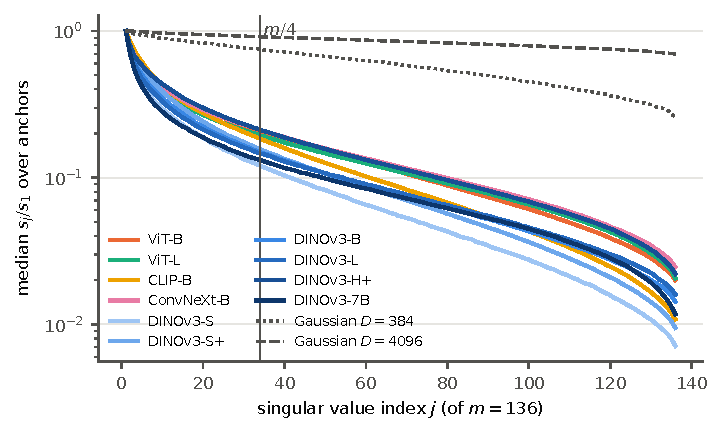
\includegraphics[width=0.72\textwidth]{figures/fig_ii_spectrum.pdf}
\caption{Median normalised singular values of the flattened in-sphere $\II^S$ at $d=16$ for ten galaxy encoders (DINOv3 sizes in shades of blue, small to large from light to dark). Grey: a Gaussian $D\times136$ matrix for the smallest and largest $D$ (recomputed with the runner's reference function, seed 0). The vertical line marks $m/4$. Source: \texttt{results/ii-rank/*.json}.}
\label{fig:ii}
\end{figure}

\paragraph{Result.} Table~\ref{tab:ii} and Figure~\ref{fig:ii}. % SOURCE: results/ii-rank/ii_rank_<enc>_d16.json via tables/tab_ii_spectrum.tex.
The in-sphere $\II$ has full rank $m$ at every anchor, with median condition numbers 41--140 against 1.4--3.9 for the Gaussian reference. The median effective rank is 22.3--42.4 of 136 (Gaussian 114--134), the participation ratio 9.9--22.1, $k_{90}$ 29--50 and $k_{99}$ 78--104. The spectrum decays smoothly, with $s_{16}/s_1=0.22$--$0.34$ and $s_{32}/s_1=0.13$--$0.22$. Under the pre-stated rule eight encoders are ``partial'' and two, the 384-wide DINOv3-S and S+, are ``low''. We therefore describe the spectrum as concentrated relative to a Gaussian matrix but full rank and graded: roughly a quarter to a third of the 136 directions hold 90\% of the squared second fundamental form. It is not low rank, and every Hessian is reachable by some normal direction at a cost set by the spectrum (Proposition~\ref{prop:pop}).

\paragraph{What this does not show.} The Gaussian matrix is a weak null: any smooth SiLU decoder produces a decaying $\II$ spectrum, and we have not fitted the decoder to data without the encoder's structure (a random-initialised decoder, a covariance-matched Gaussian cloud, column-permuted embeddings), nor estimated $\II$ without a decoder. The validation fixture has a one-dimensional in-sphere normal space, so spectrum recovery itself is unvalidated. $m$ is fixed by the chosen $d$, and we have one $d$. No non-learned embedding of the same images has been measured, so the result is about the embedding manifold as seen through this decoder, not about learning. In the DINOv3 family the median effective rank by size is 22.3, 28.3, 29.1, 29.5, 42.4 and 26.2 (S, S+, B, L, H+, 7B): there is no monotone trend, and size is confounded with width $D$ (384 to 4{,}096). % SOURCE: ii-rank JSONs (erank p50).

\paragraph{Shape versus sphere, and mean curvature.} On galaxies the in-sphere shape term dominates the probe-facing Hessian in rank (Spearman 0.95--1.00 between $\norm{K}_g$ and $\norm{K_S}_g$ over 40 encoder-label cells). % SOURCE: scaling main_xfit checks.rank_pf_full_vs_pf_tan, range 0.953-0.999.
Its density-controlled association with local $R^2$ ranges from $-0.38$ to $+0.29$ across encoders and labels, with both signs, as Eq.~\eqref{eq:resid} allows. % SOURCE: scaling main_xfit columns.pf_tan.multiscale.partial, range -0.384..+0.291.
The scalar usually reported, mean curvature, keeps only the trace of $\II$; its association with readout accuracy changes sign with the sampling on a known surface and with $d$ and the encoder on galaxies (Appendix~\ref{app:meancurv}).

% =====================================================================================================
\section{What the probe's normal component reads}
\label{sec:normal}

The workshop version reported a counterfactual: at each anchor, scale the probe's curvature term by $t$ on the anchor's neighbours and compare local $R^2$ at $t=1$ (the probe's own bend), $t=0$ (shape-flat) and $t=-1$ (reversed). This section shows what that measurement is. Least squares fixes most of its outcome, and on galaxies the decoder's quadratic carries only a minority of the probe's normal readout.

\subsection{Exact statements}

Fix an anchor with $k$ neighbours and the notation of Table~\ref{tab:notation}. The surrogate family is $\hat y_t=X(w_T+w_{\mathrm{rad}})+t\,s+c$, with the intercept $c$ refit for every $t$, where $s=p$ (variant $S$) or $s=q$ (variant $\Smodel$, the one plotted in the workshop version). Proofs are in Appendix~\ref{app:proofs}. A toy check (\texttt{scripts/prop\_check.py}: $d=2$, $D=12$, 800 neighbours) reproduces $t^*_S=1.000000$ under local least squares while $\tmodel=7.06$, and the pooled ridge identity to four decimals at $\alpha\in\{10^{-6},1,100\}$, while the per-anchor $t^*_S$ is 0.10--0.12. % SOURCE: output of paper/tmlr/scripts/prop_check.py (run 2026-10-05).

\begin{lemma}[Finite-sample identity]\label{lem:identity}
The centred residual of $\hat y_t$ is $r_c+p-t\,s$, so $\mathrm{SSE}(t)=\norm{r_c+p-t\,s}^2$ and $t^*_s=\langle r_c+p,s\rangle/\norm{s}^2$. Hence
\[
t^*_S=1+\frac{\langle r_c,p\rangle}{\norm{p}^2},\qquad \tmodel=\underbrace{\frac{\langle p,q\rangle}{\norm{q}^2}}_{\beta(p\mid q)}+\underbrace{\frac{\langle r_c,q\rangle}{\norm{q}^2}}_{\rho_r}=1+\frac{\langle r_c+e,q\rangle}{\norm{q}^2}.
\]
Moreover $\mathrm{SSE}(t)-\mathrm{SSE}(0)=\norm{s}^2(t^2-2t\,t^*)$. So $t=1$ beats shape-flat iff $t^*>\tfrac12$, $t=-1$ is worse than shape-flat iff $t^*>-\tfrac12$, and $\Delta R^2(1)=(2t^*-1)\norm{s}^2/\mathrm{SST}$. ``Help'' implies ``hurt''.
\end{lemma}

\begin{proposition}[What least squares forces]\label{prop:ls}
(a) If the probe is refit by least squares with intercept on the neighbourhood ($k>D+1$), then $t^*_S=1$ exactly, for every label including pure noise, and $\tmodel=1+\langle e,q-r_c\rangle/\norm{q}^2$, which equals 1 only if $e\perp(q-r_c)$.
(b) For a global ridge probe with intercept and penalty $\alpha\ge0$ fitted on all rows, scaling $w_S$ on all rows gives the pooled optimum $t^*_{\mathrm{pooled}}=1+\alpha\norm{w_S}^2/\norm{\tilde Xw_S}^2\ge1$, with $\tilde X$ the globally centred data; it tends to 1 as $\alpha\to0$. For any partition of the rows into patches $P$, $\sum_P\langle C_Pr,C_PXv\rangle=\alpha\,w\cdot v-\sum_Pn_P\bar r_P(\bar x_P-\bar x)\cdot v$ for every fixed direction $v$. Per anchor nothing is guaranteed: $t^*_S-1$ is that patch's share of the pooled identity plus a between-patch term, divided by the small within-patch variance $\norm{p}^2$ of a normal direction.
\end{proposition}

\begin{proposition}[Population projection and ridge shrinkage]\label{prop:pop}
Let the patch be spherically symmetric as in Eq.~\eqref{eq:sigma}, and let the manifold and label be exactly second order on it: $x(u)=x_0+Ju+\tfrac12\II(u,u)$ with $J$ orthonormal and $y=c+b^\top u+\tfrac12H(u,u)$. Let $\mathcal{R}=\{\langle v,\II\rangle:v\perp T_{x_0}M\}$. (a) Local least squares over $(w,c)$ gives $J^\top w=b$ and $K^*=\langle w_N,\II\rangle=\Pi_{\mathcal R}(H)$, the $\langle\cdot,\cdot\rangle_\Sigma$-orthogonal projection. Hence $\langle H-K^*,K^*\rangle_\Sigma=0$, scaling $K^*$ gives $t^*=1$, and the improvement condition holds automatically. In codimension one this is the normal weight $\langle H,A\rangle_\Sigma/\norm{A}^2_\Sigma$, the form of \citet[Thm.~2.4]{liu2023linear}. If $\II$ has full rank $m$, then $\mathcal R=\mathrm{Sym}^2$ and $K^*=H$. (b) With a ridge penalty $\alpha\norm{v}^2$ on the normal weight and a Gaussian patch, write the flattened $\II$ as $\mathbf{M}=\sum_js_jl_jr_j^\top$ and $h=\mathrm{flat}(H)$. Then $\mathrm{flat}(K)=\sum_jf_j\langle h,r_j\rangle r_j$ with $f_j=s_j^2/(s_j^2+\tau)$, $\tau=2\alpha/s^4$, and $t^*_{\mathrm{tensor}}=\sum_jf_jc_j^2/\sum_jf_j^2c_j^2\ge1$ with $c_j=\langle h,r_j\rangle$.
\end{proposition}

\begin{remark}\label{rem:fidelity}
In $\tmodel=\beta(p\mid q)+\rho_r$ the slope $\beta(p\mid q)=\cos(p,q)\,\norm{p}/\norm{q}$ does not change when $w_S$ is rescaled. It measures how well the decoder's quadratic reproduces the probe's own normal readout, not shrinkage. $\tmodel>1$ can arise from $\beta$ alone whenever $\norm{p}>\norm{q}$, so it is not evidence about ridge under-use of curvature.
\end{remark}

What is new relative to \citet{liu2023linear} is arbitrary codimension, the $\Sigma$-metric for non-Gaussian patches, the spectral form of ridge shrinkage (Proposition~\ref{prop:pop}b), and the finite-sample identity for a global probe (Lemma~\ref{lem:identity}, Proposition~\ref{prop:ls}). The last two are algebra. Proposition~\ref{prop:pop}(a) also shows that per-anchor expressivity is trivial when $\II$ has full rank, as it does at every galaxy anchor (Section~\ref{sec:bend}); the binding constraints are the ridge penalty and the fact that one $w$ serves every anchor. We do not have a result for the second constraint.

\subsection{Measurements}

\begin{figure}[t]
\centering
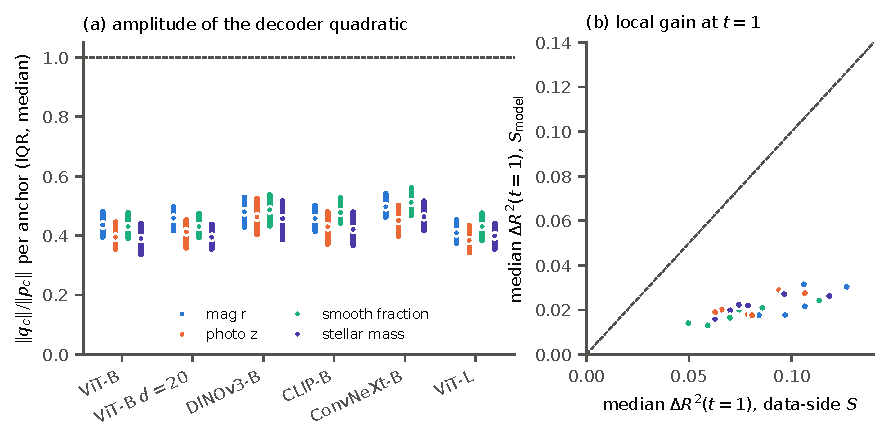
\includegraphics[width=\textwidth]{figures/fig_normal_readout.pdf}
\caption{What the probe's in-sphere normal component reads, $\alpha=100$, 512 anchors per run. (a) Per-anchor ratio of the centred amplitude of the decoder's second-order term $q$ to that of the probe's data-side in-sphere readout $p$ (bars: interquartile range; dots: median). (b) Median gain in local $R^2$ at $t=1$ over shape-flat when scaling $p$ (variant $S$) or $q$ (variant $\Smodel$); one point per run and label. Source: \texttt{notebooks/.cache/09\_physics\_normal\_scaling\_*.npz}.}
\label{fig:normal}
\end{figure}

\paragraph{Most of the normal readout is not second-order curvature.} For each anchor we compute $\norm{q}/\norm{p}=\sqrt{\norm{q}^2/\norm{p}^2}$ from the stored sums of squares of the two variants (Figure~\ref{fig:normal}a; Appendix Table~\ref{tab:normal_full}). Its median is 0.38--0.51 on the five encoders of the workshop version (24 run-label cells including ViT-B at $d=20$) and 0.38--0.51 on all ten galaxy encoders. % SOURCE: 09_physics_normal_scaling_<run>.npz, sqrt(<lab>:S_model:qq / <lab>:S:qq), medians 0.384-0.512 (tables/tab_normal_readout_full.tex); ten encoders from scaling/arrays/*__cf.npz, 0.38-0.51 (tables/tab_normal_readout_ten.tex). The outline review's 0.38-0.51 is reproduced.
If $q$ were exactly the second-order part of $p$, the remainder $e=p-q$ would carry roughly 74--85\% of the variance of the probe's in-sphere normal readout. % SOURCE: 1 - median(||q||^2/||p||^2) per cell, medians 0.148-0.262 (tab_normal_readout_full.tex); the outline review quoted 75-85%.
 This remainder contains off-manifold reconstruction residual along $w_S$, third- and higher-order terms, and the offset between the data anchor and its decoder image. We cannot yet split it, because $\langle p,q\rangle$ was not stored per anchor, so $\cos(p,q)$ and $\beta(p\mid q)$ are unknown. The local gain follows the same pattern: the median $\Delta R^2(1)$ is 0.050--0.127 for the data-side variant and 0.013--0.031 for the decoder variant (Figure~\ref{fig:normal}b). % SOURCE: same npz, medians of <lab>:S:dR2 (0.050-0.127) and <lab>:S_model:dR2 (0.013-0.031).
At $d=16$, then, most of what a probe's normal component reads on a neighbourhood is not described by the decoder's second-order model. How this share moves with $d$ is untested.

\paragraph{The data-side variant.} Scaling $p$ helps at 94--100\% of anchors on the five encoders (and 94--100\% on all ten). % SOURCE: npz <lab>:S:dR2 > 0 fraction, 0.938-1.000 (five + ViT-B d20); ten encoders 0.94-1.00 (scaling/arrays).
This uses no decoder geometry at all. Its median $t^*_S$ is 1.34--2.76 and $t^*_S>1$ at 69--100\% of anchors. % SOURCE: npz medians of <lab>:S:t_star 1.34-2.76; fraction > 1 0.69-1.00. Ten encoders: median t*_S 1.34-4.42 (scaling/arrays; DINOv3-H+ highest).
Proposition~\ref{prop:ls}(b) predicts $t^*>1$ only pooled over all rows; per anchor it predicts nothing, and we see both signs of $t^*_S-1$. So neither the help rate nor $t^*_S$ is evidence about curvature or about the label.

\paragraph{The decoder variant is an instrument check.} The published counterfactual scales $q$. It helps at 79--99\% of anchors in the ten galaxy encoders, against 21--44\% for a random in-sphere normal direction rescaled to the same centred amplitude; reversing it is worse than shape-flat at 96--100\% of anchors, and reversing the random direction at 58--81\% (Appendix Table~\ref{tab:cf}). % SOURCE: results/scaling/tab_scaling_cf.tex: help 0.79-0.99, random help 0.21-0.44, hurt 0.96-1.00, random hurt 0.58-0.81.
By Lemma~\ref{lem:identity}, help and hurt are both functions of $\tmodel$, and hurt follows from help. By Remark~\ref{rem:fidelity}, $\tmodel=\beta(p\mid q)+\rho_r$, and the gap between the fitted and the random direction mostly says that the decoder's quadratic is positively correlated with the probe's own normal readout for the fitted $w_S$ and not for a random direction, which is not part of $w$. That is a useful real-data validation of the decoder: its $\II$ is aligned with how the fitted probe actually uses its normal component. It is not evidence that the probe bends toward the label. A null that keeps $w_S$ and breaks only the geometry (an $\II$ from another anchor, or a Haar-rotated tangent frame) would isolate the decoder's contribution; it has not been run. Figure~\ref{fig:cf} reproduces the workshop figure under this reading.

\paragraph{Why $t^*$ exceeds 1.} The median $\tmodel$ is 1.4--7.6 across the ten encoders and labels at $\alpha=100$, and 0.96--1.36 with the tuned probe on five encoders. % SOURCE: tab_scaling_cf.tex t* column (1.4-7.6; DINOv3-H+ 5.5-7.6); RR REPORT Concern 2 'median t* @alpha*' 0.96-1.36.
The workshop version read $t^*>1$ as the ridge-regularised probe under-using a locally beneficial term. We withdraw that reading. With $\norm{p}/\norm{q}\approx2$--2.6 on galaxies, $\beta(p\mid q)$ alone can exceed 1, and the tuned probe changes $w_S$ and therefore $p$, $q$ and $\beta$ together. Separating $\beta$ from $\rho_r$ needs $\langle p,q\rangle$ per anchor and a sweep over $\alpha$ down to plain least squares (Section~\ref{sec:planned}).

\begin{figure}[t]
\centering
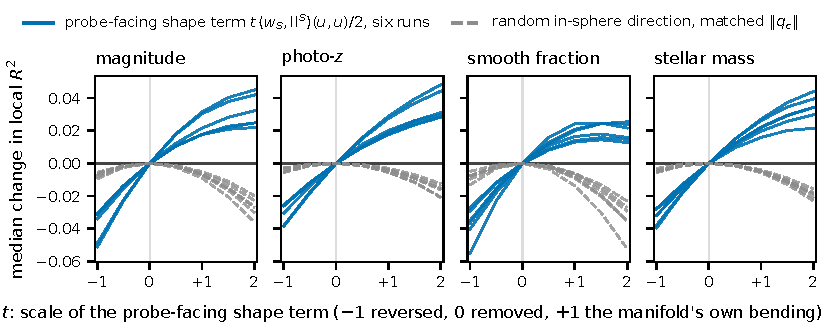
\includegraphics[width=0.85\textwidth]{figures/fig1_intervention.pdf}
\caption{Instrument check (figure from the workshop version, unchanged). At each of 512 anchors the decoder's in-sphere quadratic $\tfrac t2\langle w_S,\II^S\rangle(u,u)$ is scaled by $t$ in the local surrogate $\Smodel$; lines are the median change in local $R^2$ relative to $t=0$. Blue: one line per run (five encoders at $d=16$, ViT-B also at $d=20$). Grey dashed: a random in-sphere normal direction with matched centred amplitude. By Lemma~\ref{lem:identity} the curves are parabolas in $t$ fixed by $\tmodel$; the separation between blue and grey measures how well the decoder's quadratic tracks the fitted probe's own normal readout, not whether the probe bends toward the label.}
\label{fig:cf}
\end{figure}

% =====================================================================================================
\section{Local residual curvature and local accuracy}
\label{sec:diag}

\paragraph{Statistic.} For each anchor we compute the rank-partial Spearman correlation, over 512 anchors, between a per-anchor statistic and local $R^2$, controlling for log neighbourhood radius at five scales (16, 64, 256, 1{,}024 and 2{,}048 neighbours), local label variance and count (the multi-scale control). The workshop version called its main statistic ``curvature mismatch''. Its implementation is the emp column of Table~\ref{tab:notation}: the norm of the difference between the label's local quadratic and the quadratic fitted to the probe's predictions. It contains no $\II$; it is close to the quadratic part of the probe's local residual in the decoder chart. We therefore call it the \emph{residual-quadratic mismatch} and report it next to the decoder mismatch (dec), which the synthetic test validated, and next to the norm of the label Hessian alone.

\begin{figure}[t]
\centering
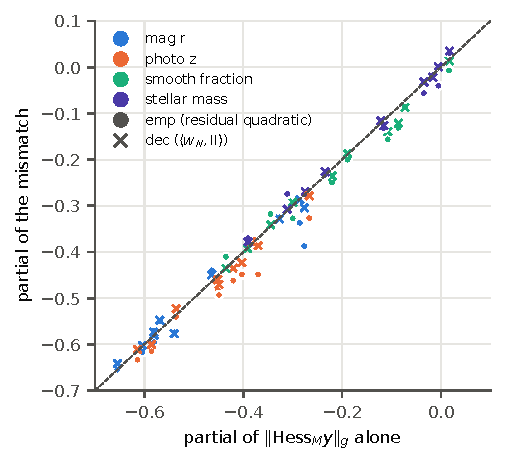
\includegraphics[width=0.48\textwidth]{figures/fig_diag_scatter.pdf}
\caption{Multi-scale partial Spearman correlation with local $R^2$ of the residual-quadratic mismatch (circles) and the decoder mismatch (crosses), against that of $\norm{\Hess y}_g$ alone; 10 galaxy encoders $\times$ 4 labels, $\alpha=100$. Source: \texttt{scaling\_\_<enc>\_\_main\_xfit.jsonl}.}
\label{fig:diag}
\end{figure}

\paragraph{The mismatch is mostly label curvature.} Figure~\ref{fig:diag} and Appendix Table~\ref{tab:diag_full}. % SOURCE: scaling/records/*__main_xfit.jsonl (multiscale partials), via tables/tab_diag_full.tex; counts printed by scripts/make_tables.py.
Across the 40 galaxy encoder-label cells, the partial of the residual-quadratic mismatch differs from that of $\norm{\Hess y}_g$ alone by at most 0.05 in 36 cells and at most 0.03 in 27, with a median gap of 0.024. The largest gaps are for ViT-B (0.11 for magnitude), the headline encoder of the workshop version. The decoder mismatch is closer still to the label-Hessian norm (within 0.05 in all 40 cells, median gap 0.008), and differs from the residual-quadratic mismatch by at most 0.08 (median 0.015). The probe-facing tensor itself, $\norm{K_S}_g$, has partials of both signs (Section~\ref{sec:bend}). So the cross-anchor association says mainly that local probe accuracy is lower where the label curves more. That is the local-regression bias of \citet{cheng2013local} and the chemistry finding of \citet{aldeghi2022roughness}, measured on foundation-model embeddings.

\begin{table}[t]
\centering\footnotesize
% SOURCE: notebooks/.cache/scaling/records/scaling__<enc>__robust.jsonl (32-block bootstrap, 2000 resamples,
% excludes_zero), ten galaxy encoders. Counts are encoders (of 10) whose 95% interval excludes zero.
% Generated by paper/tmlr/scripts/make_tables.py.
\begin{tabular}{lcccc}
\toprule
 & \multicolumn{2}{c}{residual-quadratic mismatch (emp)} & \multicolumn{2}{c}{alignment} \\
\cmidrule(lr){2-3}\cmidrule(lr){4-5}
label & $\alpha=100$ & $\alpha^*$ & $\alpha=100$ & $\alpha^*$ \\
\midrule
mag\_r & 9/10 & 10/10 & 4/10 & 8/10 \\
photo\_z & 10/10 & 10/10 & 5/10 & 7/10 \\
smooth\_fraction & 3/10 & 7/10 & 4/10 & 5/10 \\
stellar\_mass & 4/10 & 7/10 & 0/10 & 4/10 \\
\bottomrule
\end{tabular}

\caption{Encoders (of 10) in which the 95\% block-bootstrap interval (32 overlap blocks, 2{,}000 resamples) of the multi-scale partial excludes zero; galaxies, $d=16$. $\alpha^*$: validation-tuned ridge (descriptive, see text).}
\label{tab:boot}
\end{table}

\paragraph{Dependence-aware inference.} Neighbourhoods overlap, so anchor-level permutation $p$-values overstate the evidence; we quote only block-bootstrap results. % SOURCE: scaling/records/*__robust.jsonl bootstrap['32'] via tables/tab_boot_counts.tex; RR REPORT Concern 4 for the five-encoder thinned results.
For magnitude and redshift the residual-quadratic mismatch interval excludes zero in 19 of 20 encoder-label pairs at $\alpha=100$ (Table~\ref{tab:boot}); for smooth fraction and stellar mass in 7 of 20. Alignment is weaker: 4 of 10 encoders for magnitude and 5 of 10 for redshift at $\alpha=100$. On a thinned set of about 30 anchors with pairwise overlap at most 10\%, the mismatch partial for magnitude and redshift is significant in 5 of 10 encoder-label pairs on the five workshop encoders at $\alpha=100$, and 6 of 10 with the tuned probe. The ten encoders share the same galaxies, anchors and labels, so the counts measure robustness to the choice of embedding, not independent replications. \todo{state multiplicity handling (e.g.\ Bonferroni over the 20 galaxy pairs) once, with the corrected counts.}

\paragraph{Added value beyond the label's curvature.} On the five workshop encoders we add the label-Hessian norm and a local label-roughness term ($1-$ the label's linear $R^2$ in the decoder chart) to the controls, and measure the out-of-sample gain in explained variance of local $R^2$ from adding mismatch and alignment, fitting on half of the overlap blocks and scoring on the rest (20 splits). % SOURCE: RR REPORT Concern 3 tables.
At $\alpha=100$ the median held-out gain is $-0.006$ to $+0.147$, positive in 19 of 20 pairs, and its 5th percentile across splits is above zero in 9 of 20 (two of them at $+0.0001$ and $+0.0003$). % SOURCE: RR REPORT Concern 3 (alpha=100) held-out column; min -0.006 vit_large smooth_fraction, max +0.147 vit_large photo_z; p05 strictly > 0 in 9 of 20 per RR records (two print as +0.000). The outline draft's "+0.001 to +0.15" was wrong (outline review I5).
With the tuned probe the median gain is $+0.015$ to $+0.258$ with the 5th percentile above zero in 18 of 20. Adding these controls made the mismatch partial larger in magnitude in 13 of 20 pairs with the tuned probe. That is the pattern of suppression, not of over-control, so these partials need care. The 5th percentile is a quantile over overlapping splits of one dataset, not a confidence bound.

\paragraph{What has not been run.} A cross-fitted neighbourhood-residual baseline (half-A residual variance predicting half-B local $R^2$) has not been run. Local $R^2$ is computed from the residuals of the same neighbours, so we expect such a baseline to predict local $R^2$ far better than any curvature term. We therefore claim explanation, not prediction: part of local probe error has a curvature component, mostly the label's own curvature. Locally adaptive conformal intervals~\citep{tamenarvaez2026beyond} are the relevant baseline for any reliability claim and have not been compared.

\paragraph{The tuned probe.} With the validation-tuned $\alpha^*$ the galaxy partials mostly grow and the mismatch interval excludes zero for magnitude and redshift in 20 of 20 pairs (Table~\ref{tab:boot}). We present this as descriptive. $\alpha^*$ sits at the edge of the grid (0.001) in 5 of the 20 five-encoder pairs, the tuned $w_N$ was never validated on the fixture (which used $\alpha=100$), the robustness battery is not cross-fitted, and the tuned probe changes the very tensors being tested. % SOURCE: RR REPORT Concern 2 ('grid edge' rows: 5 of 20).
On molecules the tuned probe weakens several results (Section~\ref{sec:qm9}).

% =====================================================================================================
\section{Transfer to molecules: a test with a failure}
\label{sec:qm9}

We ran the same pipeline on QM9 with eight chemical language models, with $d$ set per encoder before the runs to the rounded median of four intrinsic-dimension estimates ($d=8$--11), and replicated at $d=16$. % SOURCE: results/qm9/QM9_REPORT.md 'd per encoder'.
Summary numbers follow; the full table is Appendix Table~\ref{tab:qm9}. % SOURCE: notebooks/.cache/qm9/records/*__robust.jsonl and qm9/arrays/*__cf.npz via tables/tab_qm9_full.tex; QM9_REPORT.md.

\paragraph{The residual-curvature association transfers for three of four properties.} At $\alpha=100$ the residual-quadratic mismatch partial is negative and its block-bootstrap interval excludes zero in 8 of 8 encoders for gap, $\alpha$ and $c_v$, and in 5 of 8 for $\mu$. With permutation $p$-values the counts are 8, 6, 8 and 8 of 8 at both $d_{\mathrm{run}}$ and $d=16$. On ChemFM-3B the dipole partial is $+0.11$ (permutation $p=0.015$; bootstrap interval spanning zero), a reversal of sign, and it is $+0.00$ at $d=16$, so the sign is unstable. Alignment is mostly null: positive-significant in 1, 5, 2 and 3 of 8 encoders for gap, $\mu$, $\alpha$ and $c_v$.

\paragraph{The counterfactual does not transfer.} The decoder variant beats the random direction in all 32 encoder-label pairs, but helps at only 0.28--0.74 of anchors, with help above 0.5 in 3--4 of 8 encoders per property, and the thinned-anchor sign test is significant in 1--2 of 8. The per-anchor agreement between the decoder surrogate and the actual probe is near zero (Spearman $-0.30$ to $+0.23$), while the data-side variant $S$ helps at 0.88--1.00 of anchors in every pair. The median $\norm{q}/\norm{p}$ is 0.29--0.55. % SOURCE: QM9_REPORT (c),(d) and per-encoder table; robust records surrogate.spearman -0.303..+0.233; qm9/arrays S help 0.881-1.000, ||q||/||p|| 0.289-0.549 (computed in make_tables.py).
The failure is therefore one of surrogate fidelity on molecules, not evidence that ``the effect depends on the encoder''. Why fidelity is so low is untested; third-order terms, decoder fit and duplicate embeddings (below) are conjectures.

\paragraph{The tuned probe weakens the molecular results.} With $\alpha^*$ the decoder variant helps at 0.12--0.41 of anchors for ChemBERTa, 0.56--0.60 for MoLFormer and 0.38--0.54 for ChemFM, and the median $\tmodel$ is 0.11--0.61. For ChemFM-1B and 3B the polarisability and heat-capacity mismatch partials turn positive ($+0.13$, $+0.07$, $+0.09$, $+0.11$) with bootstrap intervals spanning zero, and the held-out gain is near zero ($-0.010$ to $+0.013$). The mismatch interval excludes zero in 8, 8, 6 and 6 of 8 encoders for gap, $\mu$, $\alpha$ and $c_v$. $\alpha^*$ sits at the grid edge 0.001 in 28 of 32 pairs. % SOURCE: qm9 robust records, alpha_mode 'tuned' (printed by make_tables.py).
Conversely, at $\alpha=100$ the ChemFM probes are badly underfit (out-of-fold $R^2$ 0.27--0.63, against 0.54--0.90 tuned; widths 2{,}048 and 3{,}072 at a fixed $\alpha$), so the $\alpha=100$ ChemFM numbers describe an underfit probe.

\paragraph{Pipeline caveats.} The ChemBERTa-2 tokenizer drops bracket-atom detail, so 3{,}144 of 130{,}744 molecules (2.4\%, in 1{,}479 groups) share an embedding with another molecule in each of the five ChemBERTa models; zero nearest-neighbour distances break the TwoNN estimate (0.85--1.04). In the library used, the TLE and MLE estimators are the same formula (they agree exactly in 7 of 8 encoders), so the pre-registered $d$ is effectively the rounded mean of MLE and a second estimator; the $d=16$ replicate gives the same mismatch counts. Mean pooling includes special tokens, and only ChemFM-1B to 3B is a model-size pair. The MTR models were pretrained on descriptors that include molar refractivity, close to $\alpha$. % SOURCE: QM9_REPORT 'Duplicate embeddings', 'd per encoder' (tle == mle in 7 of 8), 'Stated limits'.

% =====================================================================================================
\section{Discussion and limitations}
\label{sec:discussion}

\paragraph{What the measurements support.} A decoder estimate of $\II$ recovers the direction of the probe-contracted shape tensor on synthetic surfaces at the real dimensions, and on galaxies its second-order term is positively related to how the fitted probe uses its normal component. The estimated $\II$ is full rank and graded at $d=16$. Most of what the probe's normal component reads at $d=16$ is not that second-order term. Least squares fixes the counterfactual's outcome in advance, and the cross-anchor curvature association is mostly the label's own curvature.

\paragraph{What a test of ``encoders bend toward physics'' would need.} The interesting question is whether a label's curvature beyond its linear part lies in the manifold's dominant bending subspace more than the curvature of equally decodable non-physical labels does. A test needs synthetic labels that share each physical label's near-OLS linear part and randomise only the residual, built intrinsically on the data's neighbourhood graph; a frame-invariant null (Haar tangent rotation); placebo labels that calibrate the leak of tangent-estimation error into the Hessian estimate; and a decision rule calibrated on surrogate-as-physical runs. Even a positive result would leave the $t=1$ versus $t=0$ comparison a least-squares fact. We have not run this test.

\paragraph{Limitations.} One galaxy sample, four galaxy labels, one $d$ for the spectrum. The label-Hessian direction is recovered only moderately on real labels (median split-half tensor cosine 0.17--0.52 across the ten encoders), % SOURCE: scaling main_xfit 'xfit' rows hessian_split_half_cos_p50, range 0.166-0.517 (0.19-0.35 on the five workshop encoders).
and the synthetic test cannot say whether this is label noise or non-smoothness at the neighbourhood scale, because its labels carry no noise. A decoder tangent tilted into the normal space leaks an $\II$-shaped error into the label-Hessian estimate that grows with the label's gradient; this has not been measured on real data. The intervention changes a local surrogate, not the encoder or the manifold. Mismatch and alignment were the pre-stated hypotheses of the workshop version; everything in Sections~\ref{sec:bend} and~\ref{sec:normal} is exploratory.

\subsection{Planned experiments (not done)}
\label{sec:planned}

None of the following has been run. Each would change a claim above; we list the claim it bears on.
\begin{enumerate}
\item \textbf{Decoder-prior nulls for the $\II$ spectrum} (Section~\ref{sec:bend}): a random-initialised decoder, an auto-encoder fitted to a covariance-matched Gaussian cloud, and one fitted to column-permuted embeddings, with seed and width subspace overlap of the top-$k$ right singular vectors against $k/m$.
\item \textbf{Decoder-free $\II$} from local quadratic regression of the ambient coordinates on the tangent chart, to bracket the spectrum from the noise side.
\item \textbf{A sweep over $d$} ($d\in\{8,12,16,20,24\}$ for ViT-B at least), reporting $\mathrm{erank}/m$, $k_{90}/m$ and $\norm{q}/\norm{p}$ against $d$, with an intrinsic-dimension estimate for reference.
\item \textbf{Ridge sweep of the data-side variant} down to plain least squares (no PCA truncation), storing $\langle p,q\rangle$ per anchor: pooled and per-anchor $t^*_S$ against $\alpha$ (Proposition~\ref{prop:ls}b predicts the pooled curve), and the split of $\tmodel$ into $\beta(p\mid q)$ and $\rho_r$.
\item \textbf{A geometry-isolating null for the decoder variant}: keep $w_S$ and use $\II$ from another anchor or a Haar-rotated tangent frame.
\item \textbf{A multi-direction validation fixture} with more than one in-sphere bending direction and a known spectrum (flat and decaying), label noise with split-half cosines, and its own Swiss-roll-style notebook.
\item \textbf{The signed magnitude ratio} $\norm{\widehat{\Hess y}}/\norm{\Hess y}$ from the tensor-fidelity records.
\item \textbf{The neighbourhood-residual baseline} and the $\norm{\Hess y}$ baseline with block-bootstrap intervals (Section~\ref{sec:diag}), and a comparison with locally adaptive conformal intervals.
\item \textbf{QM9 geometry}: the $\II$ spectrum and $\langle p,q\rangle$ on molecules, and a rerun without duplicate embeddings, to test the conjectured causes of the low surrogate fidelity.
\item \textbf{The test of Section~\ref{sec:discussion}} (surrogate labels sharing the physical label's linear part) and a non-learned embedding of the same galaxy images.
\end{enumerate}

\bibliography{references}
\bibliographystyle{tmlr}

% =====================================================================================================
\appendix

\section{Proofs}
\label{app:proofs}

\paragraph{Lemma~\ref{lem:identity}.} The probe's prediction on the neighbours is $\hat y=X(w_T+w_{\mathrm{rad}})+Xw_S+b_0$. Centring over the neighbourhood, $C(y-X(w_T+w_{\mathrm{rad}})-ts)=C(y-\hat y)+CXw_S-ts=r_c+p-ts$, using $Cs=s$ (both $p$ and $q$ are centred) and the fact that refitting $c$ removes the mean. Then $\mathrm{SSE}(t)=\norm{r_c+p-ts}^2$ is quadratic in $t$ with minimiser $\langle r_c+p,s\rangle/\norm{s}^2$. With $s=p$ this gives $1+\langle r_c,p\rangle/\norm{p}^2$; with $s=q$ and $p=q+e$ it gives $\beta(p\mid q)+\rho_r=1+\langle r_c+e,q\rangle/\norm{q}^2$. Finally $\mathrm{SSE}(t)-\mathrm{SSE}(0)=t^2\norm{s}^2-2t\langle r_c+p,s\rangle=\norm{s}^2(t^2-2t\,t^*)$, which is negative at $t=1$ iff $t^*>\tfrac12$ and positive at $t=-1$ iff $t^*>-\tfrac12$.

\paragraph{Proposition~\ref{prop:ls}(a).} Least squares with intercept on the neighbourhood makes $r_c$ orthogonal to $CXv$ for every $v$, so $\langle r_c,p\rangle=0$ and $t^*_S=1$, whatever the label. For the decoder variant, $\langle r_c,q\rangle=\langle r_c,p-e\rangle=-\langle r_c,e\rangle$ and $\langle p,q\rangle=\norm{q}^2+\langle e,q\rangle$, so $\tmodel=1+\langle e,q-r_c\rangle/\norm{q}^2$. If $D\ge k-1$ the local fit interpolates, $r=0$, and $t^*_S=1$ trivially.

\paragraph{Proposition~\ref{prop:ls}(b).} The ridge normal equations with intercept are $\tilde X^\top r=\alpha w$ with $\sum_ir_i=0$. For a fixed $v$, $\sum_ir_i(x_i-\bar x)\cdot v=\alpha w\cdot v$. Splitting the sum by patches and writing $x_i-\bar x=(x_i-\bar x_P)+(\bar x_P-\bar x)$ gives the stated decomposition. Scaling $w_S$ on all rows with a refit global intercept gives $\mathrm{SSE}(t)=\norm{r+\tilde Xw_S-t\tilde Xw_S}^2$, minimised at $1+\langle r,\tilde Xw_S\rangle/\norm{\tilde Xw_S}^2=1+\alpha\,w\cdot w_S/\norm{\tilde Xw_S}^2$, and $w\cdot w_S=\norm{w_S}^2$ because the split of $w$ is orthogonal. The real neighbourhoods overlap and do not partition the rows, and $w_S$ depends on the anchor, so the decomposition applies to one fixed $v$ and one partition at a time.

\paragraph{Eq.~\eqref{eq:sigma}.} For a spherically symmetric $u$, $\mathbb{E}u_1^2u_2^2=\tfrac13\mathbb{E}u_1^4=\lambda s^4$, so $\mathbb{E}[u^\top Au\,u^\top Bu]=\lambda s^4(\operatorname{tr}A\operatorname{tr}B+2\langle A,B\rangle_F)$ and $\mathbb{E}u^\top Au=s^2\operatorname{tr}A$. Subtracting the product of means and dividing by four gives Eq.~\eqref{eq:sigma}. For the uniform $d$-ball of radius $R$, $\mathbb{E}u_1^2=R^2/(d+2)$ and $\mathbb{E}u_1^4=3R^4/((d+2)(d+4))$, so $\lambda=(d+2)/(d+4)$.

\paragraph{Proposition~\ref{prop:pop}.} (a) On the patch, $w\cdot x+c=w\cdot x_0+c+(J^\top w)^\top u+\tfrac12\langle w_N,\II\rangle(u,u)$, since $\II$ is normal-valued. The tangent part of $w$ enters only through $J^\top w$ and the normal part only through $K=\langle w_N,\II\rangle$, and the two are chosen independently. Odd moments of $u$ vanish, so the linear and quadratic parts of the residual are uncorrelated, and the expected squared residual (after the intercept absorbs the mean) is $\norm{b-J^\top w}^2s^2+\norm{H-K}^2_\Sigma$. It is minimised by $J^\top w=b$ and $K=\Pi_{\mathcal R}(H)$ in $\langle\cdot,\cdot\rangle_\Sigma$. Orthogonality of the projection residual gives $\langle H-K^*,K^*\rangle_\Sigma=0$, so scaling $K^*$ by $t$ is optimal at $t=1$ and $2\langle H,K^*\rangle_\Sigma-\norm{K^*}^2_\Sigma=\norm{K^*}^2_\Sigma\ge0$. In codimension one $\mathcal R=\operatorname{span}(A)$. (b) In the Gaussian case $\norm{H-K}_\Sigma^2=\tfrac{s^4}{2}\norm{h-\mathbf{M}^\top v}^2$ in flattened coordinates. Minimising $\tfrac{s^4}{2}\norm{h-\mathbf M^\top v}^2+\alpha\norm{v}^2$ gives $v=(\mathbf M\mathbf M^\top+\tau I)^{-1}\mathbf Mh$ with $\tau=2\alpha/s^4$, and $\mathbf M^\top v=\sum_jf_j\langle h,r_j\rangle r_j$. Then $t^*=\langle h,\mathrm{flat}(K)\rangle/\norm{\mathrm{flat}(K)}^2=\sum f_jc_j^2/\sum f_j^2c_j^2\ge1$ because $0\le f_j\le1$. The normalisation of $\alpha$ here is per unit probability mass of the patch; a global probe is not a local ridge, so (b) does not describe it.

\clearpage
\section{Tensor-fidelity validation}
\label{app:tf}

% SOURCE: curvature-experiment/results/tensor-fidelity/REPORT.md (headline table and paper-scale table, copied by hand).
\begin{table}[h]
\centering\footnotesize\setlength{\tabcolsep}{4pt}
\begin{tabular}{llcccccc}
\toprule
noise & label & cos $K$ & cos $K_S$ & cos $\Hess y$ & $\rho$ mismatch & relerr $K_S$ & relerr $\Hess y$ \\
\midrule
0 & lin & $+1.000$ & $+0.965$ & $+0.978$ & $+0.985$ & 0.310 & 0.880 \\
0 & nonlin & $+1.000$ & $+0.963$ & $+0.916$ & $+0.991$ & 0.486 & 1.177 \\
0 & lam0 & $+1.000$ & $+0.963$ & $+0.997$ & n/i & 0.415 & 0.289 \\
0 & lam0.5 & $+1.000$ & $+0.963$ & $+0.956$ & $+0.898$ & 0.398 & 0.414 \\
0 & lam1 & $+1.000$ & $+0.965$ & $+0.951$ & $+0.923$ & 0.386 & 0.453 \\
0 & lam2 & $+1.000$ & $+0.964$ & $+0.950$ & $+0.933$ & 0.338 & 0.472 \\
\addlinespace[2pt]
0.25 & lin & $+0.999$ & $+0.843$ & $+0.977$ & $+0.984$ & 0.636 & 0.933 \\
0.25 & nonlin & $+1.000$ & $+0.675$ & $+0.914$ & $+0.991$ & 0.902 & 1.247 \\
0.25 & lam0 & $+1.000$ & $+0.803$ & $+0.965$ & n/i & 0.822 & 0.480 \\
0.25 & lam0.5 & $+1.000$ & $+0.813$ & $+0.945$ & $+0.882$ & 0.737 & 0.463 \\
0.25 & lam1 & $+1.000$ & $+0.826$ & $+0.946$ & $+0.912$ & 0.707 & 0.472 \\
0.25 & lam2 & $+1.000$ & $+0.828$ & $+0.947$ & $+0.924$ & 0.649 & 0.492 \\
\bottomrule
\end{tabular}
\caption{Tensor fidelity at paper scale ($d=16$, $D=768$, $n=86{,}471$, single seed). Medians over anchors of the cosine between estimated and true tensors; $\rho$: Spearman correlation of estimated and true decoder-mismatch norms; relerr: unsigned relative error of the norm. Noise 0.25 gives decoder variance explained 0.971. n/i: not informative (the lam0 label's true mismatch is only a ridge-shrinkage residual). The cosine of the full $K$ is dominated by the radial term, which any estimate with the right tangent plane recovers; $K_S$ is the informative column. The in-sphere normal space of the fixture is one-dimensional.}
\label{tab:tf}
\end{table}

The small fixture ($d=4$, $D=64$, 64 anchors, three seeds) passes the pre-registered line (median $K$ cosine $\ge0.8$ and mismatch Spearman $\ge0.7$ at $n=64{,}000$, noise-free) for every label, and the $K_S$ line added after review. Its full grid over $n\in\{4{,}000,16{,}000,64{,}000\}$ and four noise levels is in the report.

\clearpage
\section{What the normal component reads: full table}
\label{app:normal}

\begin{table}[h]
\centering\scriptsize\setlength{\tabcolsep}{3pt}
% SOURCE: notebooks/.cache/09_physics_normal_scaling_<enc>_<d>.npz (alpha = 100, 512 anchors, k = 2048).
% ||q||/||p|| = sqrt(<lab>:S_model:qq / <lab>:S:qq) per anchor (qq is the centred sum of squares of the scaled
% term: p = X w_S for variant S, q = (1/2)<w_S,II^S>(u,u) for S_model), median over anchors.
% t*_S, t*_model = <lab>:S:t_star, <lab>:S_model:t_star; help = fraction of anchors with dR2 > 0.
% Generated by paper/tmlr/scripts/make_tables.py.
\begin{tabular}{llccccccccc}
\toprule
 & & & & \multicolumn{3}{c}{data-side $S$ (scales $p$)} & \multicolumn{3}{c}{decoder $S_{\mathrm{model}}$ (scales $q$)} & random \\
\cmidrule(lr){5-7}\cmidrule(lr){8-10}\cmidrule(lr){11-11}
run & label & $\norm{q}/\norm{p}$ & $\norm{q}^2/\norm{p}^2$ & help & $\Delta R^2(1)$ & $t^*_S$ ($>1$) & help & $\Delta R^2(1)$ & $t^*_{\mathrm{model}}$ & help \\
\midrule
ViT-B, $d=16$ & mag\_r & 0.44 & 0.19 & 0.99 & $+0.127$ & 1.76 (0.91) & 0.97 & $+0.030$ & 2.30 & 0.26 \\
 & photo\_z & 0.39 & 0.16 & 1.00 & $+0.106$ & 2.14 (1.00) & 0.99 & $+0.028$ & 3.02 & 0.33 \\
 & smooth\_fraction & 0.43 & 0.19 & 0.94 & $+0.086$ & 1.47 (0.78) & 0.90 & $+0.021$ & 1.74 & 0.24 \\
 & stellar\_mass & 0.39 & 0.15 & 1.00 & $+0.118$ & 1.96 (0.99) & 0.96 & $+0.026$ & 2.62 & 0.29 \\
\addlinespace[2pt]
ViT-B, $d=20$ & mag\_r & 0.46 & 0.21 & 0.99 & $+0.106$ & 1.90 (0.92) & 0.99 & $+0.031$ & 2.56 & 0.24 \\
 & photo\_z & 0.41 & 0.17 & 1.00 & $+0.094$ & 2.29 (1.00) & 0.99 & $+0.029$ & 3.64 & 0.36 \\
 & smooth\_fraction & 0.43 & 0.19 & 0.95 & $+0.074$ & 1.49 (0.78) & 0.90 & $+0.020$ & 1.94 & 0.22 \\
 & stellar\_mass & 0.39 & 0.16 & 1.00 & $+0.096$ & 2.03 (0.99) & 0.97 & $+0.027$ & 3.14 & 0.32 \\
\addlinespace[2pt]
DINOv3-B, $d=16$ & mag\_r & 0.48 & 0.23 & 0.96 & $+0.080$ & 1.92 (0.91) & 0.92 & $+0.018$ & 2.05 & 0.29 \\
 & photo\_z & 0.46 & 0.21 & 1.00 & $+0.066$ & 1.87 (0.95) & 0.96 & $+0.020$ & 2.55 & 0.29 \\
 & smooth\_fraction & 0.49 & 0.24 & 1.00 & $+0.113$ & 1.53 (0.85) & 0.93 & $+0.024$ & 1.52 & 0.22 \\
 & stellar\_mass & 0.46 & 0.21 & 0.98 & $+0.063$ & 1.67 (0.86) & 0.95 & $+0.016$ & 2.07 & 0.26 \\
\addlinespace[2pt]
CLIP-B, $d=16$ & mag\_r & 0.46 & 0.21 & 0.99 & $+0.097$ & 2.13 (0.92) & 0.95 & $+0.018$ & 2.16 & 0.30 \\
 & photo\_z & 0.43 & 0.18 & 1.00 & $+0.063$ & 2.36 (0.99) & 0.99 & $+0.019$ & 3.44 & 0.36 \\
 & smooth\_fraction & 0.48 & 0.23 & 0.98 & $+0.050$ & 1.50 (0.81) & 0.92 & $+0.014$ & 1.73 & 0.25 \\
 & stellar\_mass & 0.42 & 0.18 & 1.00 & $+0.070$ & 1.96 (0.94) & 0.97 & $+0.020$ & 2.85 & 0.35 \\
\addlinespace[2pt]
ConvNeXt-B, $d=16$ & mag\_r & 0.50 & 0.25 & 0.99 & $+0.084$ & 2.13 (0.93) & 0.92 & $+0.018$ & 2.03 & 0.26 \\
 & photo\_z & 0.45 & 0.20 & 1.00 & $+0.079$ & 2.76 (1.00) & 0.99 & $+0.018$ & 2.89 & 0.28 \\
 & smooth\_fraction & 0.51 & 0.26 & 0.97 & $+0.070$ & 1.64 (0.81) & 0.88 & $+0.016$ & 1.56 & 0.23 \\
 & stellar\_mass & 0.46 & 0.21 & 1.00 & $+0.074$ & 2.33 (0.98) & 0.99 & $+0.022$ & 3.08 & 0.29 \\
\addlinespace[2pt]
ViT-L, $d=16$ & mag\_r & 0.41 & 0.17 & 0.98 & $+0.106$ & 2.09 (0.94) & 0.96 & $+0.022$ & 2.57 & 0.32 \\
 & photo\_z & 0.38 & 0.15 & 1.00 & $+0.081$ & 2.20 (0.99) & 0.97 & $+0.018$ & 3.20 & 0.34 \\
 & smooth\_fraction & 0.43 & 0.19 & 0.94 & $+0.059$ & 1.34 (0.69) & 0.79 & $+0.013$ & 1.62 & 0.25 \\
 & stellar\_mass & 0.40 & 0.16 & 1.00 & $+0.079$ & 1.92 (0.95) & 0.98 & $+0.022$ & 2.94 & 0.30 \\
\addlinespace[2pt]
\bottomrule
\end{tabular}

\caption{Per run and label, $\alpha=100$, 512 anchors. $\norm{q}/\norm{p}$: median over anchors of the ratio of centred amplitudes; $\norm{q}^2/\norm{p}^2$: its square (median). Help: fraction of anchors where $t=1$ beats $t=0$. $\Delta R^2(1)$: median. $t^*_S$: median, with the fraction of anchors where $t^*_S>1$. Random: help of the random in-sphere direction with matched centred amplitude.}
\label{tab:normal_full}
\end{table}

\begin{table}[h]
\centering\footnotesize
% SOURCE: notebooks/.cache/scaling/arrays/scaling__<enc>__cf.npz (ten galaxy encoders, d = 16, alpha = 100),
% same definitions as tab_normal_readout_full.tex; ranges are over the four labels.
% Generated by paper/tmlr/scripts/make_tables.py.
\begin{tabular}{lccc}
\toprule
encoder & median $\norm{q}/\norm{p}$ & median $t^*_S$ & help ($S$) \\
\midrule
ViT-B & 0.39--0.44 & 1.47--2.14 & 0.94--1.00 \\
ViT-L & 0.38--0.43 & 1.34--2.19 & 0.94--1.00 \\
CLIP-B & 0.42--0.48 & 1.50--2.36 & 0.98--1.00 \\
ConvNeXt-B & 0.45--0.51 & 1.64--2.76 & 0.97--1.00 \\
DINOv3-S & 0.45--0.50 & 1.56--1.90 & 0.98--1.00 \\
DINOv3-S+ & 0.47--0.49 & 1.47--2.05 & 0.96--1.00 \\
DINOv3-B & 0.46--0.49 & 1.53--1.92 & 0.96--1.00 \\
DINOv3-L & 0.44--0.50 & 1.82--2.33 & 0.97--0.99 \\
DINOv3-H+ & 0.40--0.49 & 2.68--4.42 & 0.98--1.00 \\
DINOv3-7B & 0.38--0.48 & 1.72--2.53 & 0.95--0.99 \\
\bottomrule
\end{tabular}

\caption{Ten galaxy encoders ($d=16$, $\alpha=100$): ranges over the four labels of the median amplitude ratio, the median data-side $t^*_S$, and the help fraction of the data-side variant.}
\label{tab:normal_ten}
\end{table}

\begin{table}[h]
\centering\scriptsize
% SOURCE: curvature-experiment/results/scaling/tab_scaling_cf.tex (tabular body copied verbatim by
% paper/tmlr/scripts/make_tables.py; only header labels renamed: 'model normal $S$' -> 'decoder $S_{\mathrm{model}}$').
\begin{tabular}{llccccccccc}
\toprule
 & & \multicolumn{5}{c}{decoder $S_{\mathrm{model}}$} & \multicolumn{2}{c}{random, $q$-matched} & sign test \\
encoder & label & help & hurt & $\Delta R^2(+1)$ & $\Delta R^2(-1)$ & $t^{*}$ & help & hurt & $p_{\mathrm{help}}\le$ \\
\midrule
clip\_base & mag\_r & 0.95 & 0.99 & $+0.018$ & $-0.031$ & 2.2 & 0.31 & 0.68 & $4\times 10^{-3}$ \\
 & photo\_z & 0.99 & 1.00 & $+0.019$ & $-0.026$ & 3.4 & 0.35 & 0.63 & $2\times 10^{-5}$ \\
 & smooth\_fraction & 0.92 & 0.99 & $+0.014$ & $-0.027$ & 1.7 & 0.25 & 0.69 & $2\times 10^{-4}$ \\
 & stellar\_mass & 0.97 & 1.00 & $+0.020$ & $-0.028$ & 2.9 & 0.35 & 0.68 & $5\times 10^{-7}$ \\
\addlinespace[2pt]
convnext\_base & mag\_r & 0.92 & 1.00 & $+0.018$ & $-0.031$ & 2.0 & 0.26 & 0.73 & $2\times 10^{-4}$ \\
 & photo\_z & 0.99 & 1.00 & $+0.018$ & $-0.026$ & 2.9 & 0.28 & 0.64 & $5\times 10^{-7}$ \\
 & smooth\_fraction & 0.88 & 0.98 & $+0.016$ & $-0.036$ & 1.6 & 0.23 & 0.75 & $2\times 10^{-4}$ \\
 & stellar\_mass & 0.99 & 1.00 & $+0.022$ & $-0.032$ & 3.1 & 0.29 & 0.65 & $5\times 10^{-7}$ \\
\addlinespace[2pt]
dinov3\_vits16 & mag\_r & 0.92 & 0.99 & $+0.018$ & $-0.038$ & 1.5 & 0.21 & 0.76 & $8\times 10^{-4}$ \\
 & photo\_z & 0.93 & 1.00 & $+0.013$ & $-0.022$ & 1.8 & 0.29 & 0.72 & $2\times 10^{-5}$ \\
 & smooth\_fraction & 0.85 & 0.99 & $+0.017$ & $-0.039$ & 1.4 & 0.21 & 0.79 & $4\times 10^{-3}$ \\
 & stellar\_mass & 0.83 & 0.96 & $+0.011$ & $-0.020$ & 1.6 & 0.27 & 0.74 & $2\times 10^{-5}$ \\
\addlinespace[2pt]
dinov3\_vits16plus & mag\_r & 0.89 & 0.99 & $+0.017$ & $-0.034$ & 1.6 & 0.28 & 0.76 & $4\times 10^{-3}$ \\
 & photo\_z & 0.94 & 0.99 & $+0.017$ & $-0.029$ & 2.0 & 0.27 & 0.69 & $2\times 10^{-4}$ \\
 & smooth\_fraction & 0.84 & 0.99 & $+0.017$ & $-0.040$ & 1.4 & 0.23 & 0.81 & $2\times 10^{-5}$ \\
 & stellar\_mass & 0.89 & 0.99 & $+0.015$ & $-0.029$ & 1.7 & 0.25 & 0.71 & $2\times 10^{-4}$ \\
\addlinespace[2pt]
dinov3\_vitb16 & mag\_r & 0.92 & 0.99 & $+0.018$ & $-0.031$ & 2.0 & 0.29 & 0.71 & $8\times 10^{-4}$ \\
 & photo\_z & 0.96 & 0.99 & $+0.020$ & $-0.030$ & 2.6 & 0.29 & 0.71 & $2\times 10^{-5}$ \\
 & smooth\_fraction & 0.93 & 1.00 & $+0.024$ & $-0.055$ & 1.5 & 0.22 & 0.78 & $2\times 10^{-4}$ \\
 & stellar\_mass & 0.95 & 1.00 & $+0.016$ & $-0.028$ & 2.1 & 0.26 & 0.74 & $5\times 10^{-7}$ \\
\addlinespace[2pt]
dinov3\_vitl16 & mag\_r & 0.97 & 1.00 & $+0.022$ & $-0.033$ & 2.5 & 0.26 & 0.72 & $5\times 10^{-4}$ \\
 & photo\_z & 0.94 & 0.98 & $+0.015$ & $-0.021$ & 3.1 & 0.33 & 0.64 & $7\times 10^{-5}$ \\
 & smooth\_fraction & 0.91 & 1.00 & $+0.025$ & $-0.044$ & 1.9 & 0.28 & 0.76 & $7\times 10^{-5}$ \\
 & stellar\_mass & 0.95 & 0.99 & $+0.016$ & $-0.023$ & 3.2 & 0.34 & 0.68 & $6\times 10^{-6}$ \\
\addlinespace[2pt]
dinov3\_vith16plus & mag\_r & 0.98 & 1.00 & $+0.017$ & $-0.022$ & 5.5 & 0.38 & 0.61 & $2\times 10^{-5}$ \\
 & photo\_z & 0.98 & 0.99 & $+0.017$ & $-0.020$ & 7.5 & 0.44 & 0.58 & $2\times 10^{-4}$ \\
 & smooth\_fraction & 0.95 & 0.99 & $+0.022$ & $-0.033$ & 3.2 & 0.36 & 0.68 & $5\times 10^{-7}$ \\
 & stellar\_mass & 0.98 & 0.99 & $+0.019$ & $-0.021$ & 7.6 & 0.41 & 0.59 & $2\times 10^{-5}$ \\
\addlinespace[2pt]
dinov3\_vit7b16 & mag\_r & 0.97 & 1.00 & $+0.027$ & $-0.039$ & 2.9 & 0.30 & 0.70 & $3\times 10^{-5}$ \\
 & photo\_z & 0.97 & 1.00 & $+0.020$ & $-0.029$ & 3.5 & 0.35 & 0.65 & $3\times 10^{-5}$ \\
 & smooth\_fraction & 0.94 & 0.99 & $+0.035$ & $-0.062$ & 2.3 & 0.25 & 0.71 & $3\times 10^{-4}$ \\
 & stellar\_mass & 0.90 & 1.00 & $+0.016$ & $-0.027$ & 3.3 & 0.33 & 0.67 & $3\times 10^{-5}$ \\
\addlinespace[2pt]
vit\_base & mag\_r & 0.97 & 1.00 & $+0.030$ & $-0.051$ & 2.3 & 0.26 & 0.80 & $3\times 10^{-4}$ \\
 & photo\_z & 0.99 & 0.99 & $+0.028$ & $-0.038$ & 3.0 & 0.33 & 0.68 & $3\times 10^{-5}$ \\
 & smooth\_fraction & 0.90 & 1.00 & $+0.021$ & $-0.040$ & 1.7 & 0.25 & 0.78 & $3\times 10^{-5}$ \\
 & stellar\_mass & 0.96 & 0.99 & $+0.026$ & $-0.039$ & 2.6 & 0.28 & 0.70 & $3\times 10^{-5}$ \\
\addlinespace[2pt]
vit\_large & mag\_r & 0.96 & 0.99 & $+0.022$ & $-0.034$ & 2.6 & 0.32 & 0.73 & $2\times 10^{-6}$ \\
 & photo\_z & 0.97 & 0.99 & $+0.017$ & $-0.025$ & 3.2 & 0.34 & 0.66 & $2\times 10^{-6}$ \\
 & smooth\_fraction & 0.79 & 0.97 & $+0.013$ & $-0.029$ & 1.6 & 0.25 & 0.77 & $4\times 10^{-4}$ \\
 & stellar\_mass & 0.98 & 1.00 & $+0.022$ & $-0.032$ & 3.0 & 0.29 & 0.67 & $2\times 10^{-6}$ \\
\addlinespace[2pt]
\bottomrule
\end{tabular}

\caption{Decoder-variant counterfactual on ten galaxy encoders at $d=16$, $\alpha=100$ (from the scaling report). Help: $t=1$ beats shape-flat; hurt: $t=-1$ worse than shape-flat; median $\Delta R^2$ at $t=\pm1$ and median $\tmodel$; the same for a random in-sphere direction rescaled to the same centred amplitude; one-sided sign-test bound for help on a maximal set of anchors with pairwise overlap at most 5\% of $k$. By Lemma~\ref{lem:identity} help and hurt are functions of $\tmodel$.}
\label{tab:cf}
\end{table}

\clearpage
\section{Residual curvature: full tables}
\label{app:diag}

\begin{table}[h]
\centering\scriptsize\setlength{\tabcolsep}{3pt}
% SOURCE: notebooks/.cache/scaling/records/scaling__<enc>__main_xfit.jsonl, rows 'result' (columns
% hess_mismatch_emp, hess_mismatch_dec, hess_label, align_cos_tan; key 'multiscale') and rows 'xfit'
% (hess_mismatch_dec and hess_label, fitA_scoreB); bootstrap flags from scaling__<enc>__robust.jsonl,
% bootstrap['32'][col]['excludes_zero'], alpha_mode published (alpha=100) and tuned (alpha*).
% NOTE: the cross-fit 'mismatch' columns of the ML4PS appendix (Tables B and C there) are hess_mismatch_dec
% (the xfit rows store only dec, align and hess_label), while its main-table mismatch is hess_mismatch_emp.
% The sanity review says every real-data table uses emp; the records say the cross-fit tables use dec.
% Generated by paper/tmlr/scripts/make_tables.py.
\begin{tabular}{llcccccccc}
\toprule
 & & \multicolumn{4}{c}{multi-scale partial, $\alpha=100$} & \multicolumn{2}{c}{cross-fit (A$\to$B)} & \multicolumn{2}{c}{boot.\ CI excl.\ 0, emp} \\
\cmidrule(lr){3-6}\cmidrule(lr){7-8}\cmidrule(lr){9-10}
encoder & label & emp & dec & $\norm{\operatorname{Hess}_M y}_g$ & align & dec & $\norm{\operatorname{Hess}_M y}_g$ & $\alpha=100$ & $\alpha^*$ \\
\midrule
ViT-B & mag\_r & $-0.39$ & $-0.30$ & $-0.28$ & $+0.35$ & $-0.38$ & $-0.36$ & y & y \\
 & photo\_z & $-0.45$ & $-0.39$ & $-0.37$ & $+0.26$ & $-0.42$ & $-0.41$ & y & y \\
 & smooth\_fraction & $-0.09^{*}$ & $-0.09^{*}$ & $-0.07^{*}$ & $+0.19$ & $-0.10$ & $-0.10$ & n & n \\
 & stellar\_mass & $-0.04^{*}$ & $+0.00^{*}$ & $-0.01^{*}$ & $+0.01^{*}$ & $+0.01^{*}$ & $+0.00^{*}$ & n & n \\
\addlinespace[2pt]
ViT-L & mag\_r & $-0.44$ & $-0.45$ & $-0.46$ & $+0.13$ & $-0.46$ & $-0.47$ & y & y \\
 & photo\_z & $-0.46$ & $-0.44$ & $-0.42$ & $+0.14$ & $-0.43$ & $-0.43$ & y & y \\
 & smooth\_fraction & $-0.01^{*}$ & $+0.01^{*}$ & $+0.02^{*}$ & $+0.14$ & $-0.03^{*}$ & $-0.03^{*}$ & n & n \\
 & stellar\_mass & $-0.02^{*}$ & $-0.02^{*}$ & $-0.02^{*}$ & $-0.02^{*}$ & $-0.06^{*}$ & $-0.06^{*}$ & n & y \\
\addlinespace[2pt]
CLIP-B & mag\_r & $-0.34$ & $-0.29$ & $-0.29$ & $+0.33$ & $-0.28$ & $-0.28$ & y & y \\
 & photo\_z & $-0.45$ & $-0.42$ & $-0.40$ & $+0.06^{*}$ & $-0.40$ & $-0.39$ & y & y \\
 & smooth\_fraction & $-0.25$ & $-0.24$ & $-0.22$ & $+0.24$ & $-0.22$ & $-0.21$ & n & y \\
 & stellar\_mass & $-0.13$ & $-0.12$ & $-0.12$ & $-0.01^{*}$ & $-0.14$ & $-0.14$ & n & n \\
\addlinespace[2pt]
ConvNeXt-B & mag\_r & $-0.32$ & $-0.33$ & $-0.33$ & $+0.21$ & $-0.36$ & $-0.37$ & n & y \\
 & photo\_z & $-0.48$ & $-0.46$ & $-0.45$ & $+0.22$ & $-0.46$ & $-0.46$ & y & y \\
 & smooth\_fraction & $-0.20$ & $-0.19$ & $-0.19$ & $+0.04^{*}$ & $-0.15$ & $-0.16$ & n & n \\
 & stellar\_mass & $-0.06^{*}$ & $-0.03^{*}$ & $-0.03^{*}$ & $+0.07^{*}$ & $-0.05^{*}$ & $-0.05^{*}$ & n & y \\
\addlinespace[2pt]
DINOv3-S & mag\_r & $-0.62$ & $-0.60$ & $-0.60$ & $+0.21$ & $-0.62$ & $-0.63$ & y & y \\
 & photo\_z & $-0.63$ & $-0.61$ & $-0.61$ & $-0.01^{*}$ & $-0.58$ & $-0.58$ & y & y \\
 & smooth\_fraction & $-0.13$ & $-0.12$ & $-0.09$ & $+0.31$ & $-0.16$ & $-0.14$ & n & y \\
 & stellar\_mass & $-0.23$ & $-0.23$ & $-0.23$ & $+0.01^{*}$ & $-0.24$ & $-0.25$ & y & y \\
\addlinespace[2pt]
DINOv3-S+ & mag\_r & $-0.59$ & $-0.58$ & $-0.58$ & $+0.18$ & $-0.57$ & $-0.57$ & y & y \\
 & photo\_z & $-0.54$ & $-0.52$ & $-0.54$ & $+0.12$ & $-0.50$ & $-0.51$ & y & y \\
 & smooth\_fraction & $-0.16$ & $-0.14$ & $-0.11$ & $+0.25$ & $-0.18$ & $-0.15$ & n & y \\
 & stellar\_mass & $-0.13$ & $-0.13$ & $-0.12$ & $+0.12$ & $-0.12$ & $-0.12$ & n & y \\
\addlinespace[2pt]
DINOv3-B & mag\_r & $-0.57$ & $-0.58$ & $-0.54$ & $+0.53$ & $-0.60$ & $-0.57$ & y & y \\
 & photo\_z & $-0.61$ & $-0.60$ & $-0.59$ & $+0.33$ & $-0.56$ & $-0.55$ & y & y \\
 & smooth\_fraction & $-0.33$ & $-0.29$ & $-0.30$ & $-0.02^{*}$ & $-0.32$ & $-0.33$ & n & y \\
 & stellar\_mass & $+0.03^{*}$ & $+0.04^{*}$ & $+0.02^{*}$ & $-0.05^{*}$ & $+0.03^{*}$ & $+0.03^{*}$ & n & n \\
\addlinespace[2pt]
DINOv3-L & mag\_r & $-0.55$ & $-0.55$ & $-0.57$ & $+0.01^{*}$ & $-0.52$ & $-0.54$ & y & y \\
 & photo\_z & $-0.49$ & $-0.47$ & $-0.45$ & $+0.18$ & $-0.49$ & $-0.48$ & y & y \\
 & smooth\_fraction & $-0.41$ & $-0.44$ & $-0.44$ & $+0.10$ & $-0.44$ & $-0.44$ & y & y \\
 & stellar\_mass & $-0.27$ & $-0.27$ & $-0.27$ & $-0.05^{*}$ & $-0.27$ & $-0.27$ & y & y \\
\addlinespace[2pt]
DINOv3-H+ & mag\_r & $-0.57$ & $-0.57$ & $-0.58$ & $-0.08^{*}$ & $-0.57$ & $-0.58$ & y & y \\
 & photo\_z & $-0.33$ & $-0.28$ & $-0.27$ & $+0.05^{*}$ & $-0.23$ & $-0.23$ & y & y \\
 & smooth\_fraction & $-0.32$ & $-0.34$ & $-0.34$ & $+0.05^{*}$ & $-0.35$ & $-0.35$ & y & y \\
 & stellar\_mass & $-0.27$ & $-0.31$ & $-0.31$ & $-0.13$ & $-0.27$ & $-0.28$ & y & y \\
\addlinespace[2pt]
DINOv3-7B & mag\_r & $-0.65$ & $-0.64$ & $-0.65$ & $+0.15$ & $-0.65$ & $-0.66$ & y & y \\
 & photo\_z & $-0.37$ & $-0.38$ & $-0.38$ & $+0.17$ & $-0.37$ & $-0.37$ & y & y \\
 & smooth\_fraction & $-0.36$ & $-0.39$ & $-0.39$ & $+0.10$ & $-0.43$ & $-0.43$ & y & y \\
 & stellar\_mass & $-0.37$ & $-0.38$ & $-0.39$ & $-0.05^{*}$ & $-0.38$ & $-0.39$ & y & y \\
\addlinespace[2pt]
\bottomrule
\end{tabular}

\caption{Ten galaxy encoders, $d=16$, 512 anchors, multi-scale control. Rank-partial Spearman correlations with local $R^2$ of the residual-quadratic mismatch (emp), the decoder mismatch (dec), the label-Hessian norm alone and the alignment; cross-fitted (Hessian fitted on one half of each neighbourhood, local $R^2$ scored on the other) for dec and the label-Hessian norm; whether the 32-block bootstrap interval of emp excludes zero at $\alpha=100$ and $\alpha^*$. $^*$: permutation $p\ge0.05$ (anchor-level, shown for orientation only). The cross-fitted ``mismatch'' columns of the workshop version's appendix are the dec column here.}
\label{tab:diag_full}
\end{table}

\begin{table}[h]
\centering\scriptsize
% SOURCE: curvature-experiment/results/scaling/tab_scaling_robust.tex (tabular body copied verbatim by
% paper/tmlr/scripts/make_tables.py; only header labels renamed: ).
\begin{tabular}{llcccc}
\toprule
 & & \multicolumn{2}{c}{mismatch} & \multicolumn{2}{c}{alignment} \\
encoder & label & min--max & sign flips & min--max & sign flips \\
\midrule
clip\_base & mag\_r & $[-0.34, -0.33]$ & 0 & $[+0.30, +0.33]$ & 0 \\
 & photo\_z & $[-0.46, -0.45]$ & 0 & $[+0.02, +0.06]$ & 0 \\
 & smooth\_fraction & $[-0.27, -0.24]$ & 0 & $[+0.17, +0.24]$ & 0 \\
 & stellar\_mass & $[-0.13, -0.09]$ & 0 & $[-0.01, +0.14]$ & 2 \\
\addlinespace[2pt]
convnext\_base & mag\_r & $[-0.34, -0.32]$ & 0 & $[+0.14, +0.21]$ & 0 \\
 & photo\_z & $[-0.48, -0.48]$ & 0 & $[+0.15, +0.22]$ & 0 \\
 & smooth\_fraction & $[-0.21, -0.18]$ & 0 & $[+0.04, +0.09]$ & 0 \\
 & stellar\_mass & $[-0.06, -0.04]$ & 0 & $[-0.02, +0.07]$ & 1 \\
\addlinespace[2pt]
dinov3\_vits16 & mag\_r & $[-0.62, -0.62]$ & 0 & $[+0.19, +0.21]$ & 0 \\
 & photo\_z & $[-0.64, -0.62]$ & 0 & $[-0.01, +0.06]$ & 2 \\
 & smooth\_fraction & $[-0.13, -0.12]$ & 0 & $[+0.29, +0.32]$ & 0 \\
 & stellar\_mass & $[-0.24, -0.23]$ & 0 & $[+0.01, +0.06]$ & 0 \\
\addlinespace[2pt]
dinov3\_vits16plus & mag\_r & $[-0.60, -0.58]$ & 0 & $[+0.18, +0.26]$ & 0 \\
 & photo\_z & $[-0.54, -0.53]$ & 0 & $[+0.12, +0.18]$ & 0 \\
 & smooth\_fraction & $[-0.16, -0.12]$ & 0 & $[+0.18, +0.29]$ & 0 \\
 & stellar\_mass & $[-0.15, -0.13]$ & 0 & $[+0.08, +0.14]$ & 0 \\
\addlinespace[2pt]
dinov3\_vitb16 & mag\_r & $[-0.57, -0.56]$ & 0 & $[+0.53, +0.56]$ & 0 \\
 & photo\_z & $[-0.62, -0.61]$ & 0 & $[+0.27, +0.33]$ & 0 \\
 & smooth\_fraction & $[-0.34, -0.33]$ & 0 & $[-0.07, +0.05]$ & 1 \\
 & stellar\_mass & $[+0.02, +0.04]$ & 0 & $[-0.14, -0.05]$ & 0 \\
\addlinespace[2pt]
dinov3\_vitl16 & mag\_r & $[-0.56, -0.52]$ & 0 & $[+0.01, +0.13]$ & 0 \\
 & photo\_z & $[-0.50, -0.48]$ & 0 & $[+0.16, +0.22]$ & 0 \\
 & smooth\_fraction & $[-0.44, -0.41]$ & 0 & $[+0.01, +0.10]$ & 0 \\
 & stellar\_mass & $[-0.27, -0.24]$ & 0 & $[-0.05, +0.06]$ & 2 \\
\addlinespace[2pt]
dinov3\_vith16plus & mag\_r & $[-0.58, -0.57]$ & 0 & $[-0.08, +0.06]$ & 2 \\
 & photo\_z & $[-0.34, -0.33]$ & 0 & $[+0.05, +0.17]$ & 0 \\
 & smooth\_fraction & $[-0.32, -0.30]$ & 0 & $[+0.05, +0.13]$ & 0 \\
 & stellar\_mass & $[-0.29, -0.27]$ & 0 & $[-0.13, -0.05]$ & 0 \\
\addlinespace[2pt]
dinov3\_vit7b16 & mag\_r & $[-0.66, -0.65]$ & 0 & $[+0.10, +0.15]$ & 0 \\
 & photo\_z & $[-0.42, -0.37]$ & 0 & $[+0.02, +0.17]$ & 0 \\
 & smooth\_fraction & $[-0.39, -0.36]$ & 0 & $[+0.07, +0.11]$ & 0 \\
 & stellar\_mass & $[-0.37, -0.33]$ & 0 & $[-0.05, +0.02]$ & 2 \\
\addlinespace[2pt]
vit\_base & mag\_r & $[-0.39, -0.34]$ & 0 & $[+0.31, +0.37]$ & 0 \\
 & photo\_z & $[-0.45, -0.42]$ & 0 & $[+0.24, +0.26]$ & 0 \\
 & smooth\_fraction & $[-0.09, -0.05]$ & 0 & $[+0.09, +0.19]$ & 0 \\
 & stellar\_mass & $[-0.04, +0.03]$ & 2 & $[-0.03, +0.03]$ & 1 \\
\addlinespace[2pt]
vit\_large & mag\_r & $[-0.44, -0.42]$ & 0 & $[+0.13, +0.16]$ & 0 \\
 & photo\_z & $[-0.47, -0.45]$ & 0 & $[+0.14, +0.19]$ & 0 \\
 & smooth\_fraction & $[-0.02, -0.01]$ & 0 & $[+0.13, +0.18]$ & 0 \\
 & stellar\_mass & $[-0.03, -0.02]$ & 0 & $[-0.03, +0.03]$ & 1 \\
\addlinespace[2pt]
\bottomrule
\end{tabular}

\caption{Decoder-seed stability (from the scaling report): range of the emp mismatch and alignment partials over decoder seeds 0, 1 and 2, and the number of refits whose sign differs from seed 0.}
\label{tab:seeds}
\end{table}

\clearpage
\section{QM9: full table}
\label{app:qm9}

\begin{table}[h]
\centering\scriptsize\setlength{\tabcolsep}{2.5pt}
% SOURCE: notebooks/.cache/qm9/records/scaling__<enc>__robust.jsonl (rows 'result', alpha_mode published
% = alpha 100 and tuned = alpha*; global_oof_r2, partials.published_controls.hess_mismatch_emp (permutation p),
% bootstrap['32'] excludes_zero, cf.S_model help and t_star, surrogate.spearman); help of the data-side
% variant S and ||q||/||p|| from notebooks/.cache/qm9/arrays/scaling__<enc>__cf.npz (alpha = 100).
% Generated by paper/tmlr/scripts/make_tables.py.
\begin{tabular}{llcccccccccc}
\toprule
 & & \multicolumn{2}{c}{OOF $R^2$} & \multicolumn{2}{c}{mismatch (emp)} & \multicolumn{2}{c}{help $S_{\mathrm{model}}$} & \multicolumn{2}{c}{$t^*_{\mathrm{model}}$} & & \\
\cmidrule(lr){3-4}\cmidrule(lr){5-6}\cmidrule(lr){7-8}\cmidrule(lr){9-10}
encoder & label & $100$ & $\alpha^*$ & $100$ & $\alpha^*$ & $100$ & $\alpha^*$ & $100$ & $\alpha^*$ & $\rho_{\mathrm{sur}}$ & help $S$ \\
\midrule
ChemBERTa-10M-MLM & gap & 0.76 & 0.83 & $-0.33$$^\dagger$ & $-0.40$$^\dagger$ & 0.44 & 0.37 & 0.41 & 0.35 & $-0.00$ & 0.99 \\
 & mu & 0.38 & 0.47 & $-0.17$$^\dagger$ & $-0.31$$^\dagger$ & 0.46 & 0.39 & 0.43 & 0.36 & $+0.20$ & 0.93 \\
 & alpha & 0.69 & 0.84 & $-0.44$$^\dagger$ & $-0.37$$^\dagger$ & 0.48 & 0.28 & 0.48 & 0.30 & $-0.06$ & 1.00 \\
 & cv & 0.78 & 0.89 & $-0.50$$^\dagger$ & $-0.40$$^\dagger$ & 0.48 & 0.30 & 0.47 & 0.34 & $-0.08$ & 1.00 \\
\addlinespace[2pt]
ChemBERTa-77M-MLM & gap & 0.75 & 0.81 & $-0.36$$^\dagger$ & $-0.43$$^\dagger$ & 0.53 & 0.38 & 0.56 & 0.38 & $-0.04$ & 1.00 \\
 & mu & 0.40 & 0.47 & $-0.17$$^\dagger$ & $-0.31$$^\dagger$ & 0.55 & 0.41 & 0.58 & 0.38 & $+0.12$ & 0.95 \\
 & alpha & 0.68 & 0.81 & $-0.35$$^\dagger$ & $-0.31$$^\dagger$ & 0.44 & 0.29 & 0.41 & 0.30 & $-0.00$ & 1.00 \\
 & cv & 0.76 & 0.87 & $-0.30$$^\dagger$ & $-0.26$$^\dagger$ & 0.52 & 0.40 & 0.55 & 0.41 & $-0.11$ & 1.00 \\
\addlinespace[2pt]
ChemBERTa-5M-MTR & gap & 0.80 & 0.86 & $-0.44$$^\dagger$ & $-0.44$$^\dagger$ & 0.37 & 0.30 & 0.23 & 0.17 & $+0.03$ & 0.94 \\
 & mu & 0.45 & 0.55 & $-0.14$$^\dagger$ & $-0.21$$^\dagger$ & 0.37 & 0.29 & 0.21 & 0.20 & $+0.16$ & 0.88 \\
 & alpha & 0.66 & 0.87 & $-0.21$$^\dagger$ & $-0.30$$^\dagger$ & 0.29 & 0.12 & 0.26 & 0.12 & $-0.20$ & 1.00 \\
 & cv & 0.76 & 0.91 & $-0.39$$^\dagger$ & $-0.33$$^\dagger$ & 0.33 & 0.13 & 0.30 & 0.11 & $-0.29$ & 1.00 \\
\addlinespace[2pt]
ChemBERTa-10M-MTR & gap & 0.82 & 0.87 & $-0.51$$^\dagger$ & $-0.50$$^\dagger$ & 0.28 & 0.22 & 0.11 & 0.11 & $+0.15$ & 0.90 \\
 & mu & 0.46 & 0.56 & $-0.33$$^\dagger$ & $-0.27$$^\dagger$ & 0.29 & 0.23 & 0.15 & 0.18 & $+0.15$ & 0.89 \\
 & alpha & 0.76 & 0.90 & $-0.27$$^\dagger$ & $-0.31$$^\dagger$ & 0.35 & 0.19 & 0.32 & 0.23 & $-0.21$ & 1.00 \\
 & cv & 0.81 & 0.93 & $-0.40$$^\dagger$ & $-0.44$$^\dagger$ & 0.36 & 0.24 & 0.33 & 0.25 & $-0.22$ & 1.00 \\
\addlinespace[2pt]
ChemBERTa-77M-MTR & gap & 0.77 & 0.87 & $-0.30$$^\dagger$ & $-0.49$$^\dagger$ & 0.30 & 0.24 & 0.10 & 0.15 & $-0.03$ & 0.90 \\
 & mu & 0.39 & 0.55 & $-0.09$ & $-0.30$$^\dagger$ & 0.34 & 0.23 & 0.07 & 0.15 & $+0.01$ & 0.89 \\
 & alpha & 0.72 & 0.90 & $-0.22$$^\dagger$ & $-0.38$$^\dagger$ & 0.45 & 0.34 & 0.37 & 0.34 & $-0.09$ & 1.00 \\
 & cv & 0.75 & 0.93 & $-0.31$$^\dagger$ & $-0.38$$^\dagger$ & 0.47 & 0.36 & 0.44 & 0.33 & $-0.30$ & 1.00 \\
\addlinespace[2pt]
MoLFormer-XL & gap & 0.73 & 0.83 & $-0.43$$^\dagger$ & $-0.51$$^\dagger$ & 0.71 & 0.56 & 0.85 & 0.60 & $+0.05$ & 0.99 \\
 & mu & 0.39 & 0.51 & $-0.33$$^\dagger$ & $-0.39$$^\dagger$ & 0.68 & 0.58 & 0.75 & 0.59 & $+0.14$ & 0.98 \\
 & alpha & 0.65 & 0.81 & $-0.65$$^\dagger$ & $-0.51$$^\dagger$ & 0.74 & 0.58 & 0.87 & 0.59 & $+0.10$ & 1.00 \\
 & cv & 0.76 & 0.87 & $-0.66$$^\dagger$ & $-0.51$$^\dagger$ & 0.66 & 0.60 & 0.79 & 0.60 & $-0.03$ & 1.00 \\
\addlinespace[2pt]
ChemFM-1B & gap & 0.53 & 0.84 & $-0.16$$^\dagger$ & $-0.33$$^\dagger$ & 0.64 & 0.45 & 1.13 & 0.46 & $+0.16$ & 0.98 \\
 & mu & 0.27 & 0.54 & $+0.05^{*}$ & $-0.26$$^\dagger$ & 0.60 & 0.52 & 0.91 & 0.52 & $+0.23$ & 0.93 \\
 & alpha & 0.49 & 0.86 & $-0.22$$^\dagger$ & $+0.13$ & 0.54 & 0.38 & 0.58 & 0.38 & $-0.06$ & 1.00 \\
 & cv & 0.63 & 0.90 & $-0.34$$^\dagger$ & $+0.06^{*}$ & 0.60 & 0.41 & 0.73 & 0.41 & $-0.12$ & 1.00 \\
\addlinespace[2pt]
ChemFM-3B & gap & 0.51 & 0.85 & $-0.13$$^\dagger$ & $-0.27$$^\dagger$ & 0.71 & 0.54 & 1.47 & 0.55 & $+0.15$ & 0.99 \\
 & mu & 0.27 & 0.54 & $+0.11$ & $-0.19$$^\dagger$ & 0.59 & 0.54 & 0.75 & 0.54 & $+0.16$ & 0.92 \\
 & alpha & 0.45 & 0.87 & $-0.24$$^\dagger$ & $+0.09$ & 0.51 & 0.38 & 0.52 & 0.36 & $+0.02$ & 1.00 \\
 & cv & 0.61 & 0.90 & $-0.26$$^\dagger$ & $+0.11$ & 0.57 & 0.49 & 0.70 & 0.49 & $+0.00$ & 1.00 \\
\addlinespace[2pt]
\bottomrule
\end{tabular}

\caption{QM9, eight encoders at their pre-stated $d$, 512 anchors, $k=2{,}048$. OOF $R^2$: global out-of-fold $R^2$ at $\alpha=100$ and at $\alpha^*$. Mismatch: residual-quadratic partial with the published controls ($^*$: permutation $p\ge0.05$; $^\dagger$: 32-block bootstrap interval excludes zero). Help and $\tmodel$: decoder variant. $\rho_{\mathrm{sur}}$: per-anchor Spearman correlation between the local $R^2$ of the decoder surrogate and of the actual probe at $t=1$ ($\alpha=100$). Help $S$: data-side variant ($\alpha=100$).}
\label{tab:qm9}
\end{table}

\clearpage
\section{Shape term, sphere term and mean curvature}
\label{app:meancurv}

% SOURCE: paper/latex/main.tex Appendix E and Table tab:meancurv (ML4PS, record-verified values per its own comment). Not re-derived here.
The mean-curvature vector of the decoder surface is $H=\operatorname{tr}_g\II$. Alongside Eq.~\eqref{eq:hess}, $\Delta_M(w\cdot x)=\langle w,H\rangle$: the Laplacian of a linear readout sees only the trace of $\II$, its Hessian the whole tensor. On the unit sphere every $d$-submanifold has the universal radial mean-curvature component $-d\,\hat x$; differentiating the projected decoder splits $H=-d\,\hat x+\Htan$ exactly, and the radial part is $-16$ to within $3\times10^{-9}$ at ViT-B anchors. % SOURCE: scaling__vit_base__main_xfit.jsonl checks.H_rad_median = -16.0000000023.

\emph{Validation surface.} At $D=768$ the in-sphere surface $G(z)=Q\,\mathrm{normalize}([\phi(z);0.8\,h(z);0\ldots])$ ($\phi$ inverse stereographic $\mathbb{R}^{16}\to S^{16}$, $h$ four Gaussian bumps, $Q$ a rotation) has closed-form curvature; the decoder's $\Htan$ gives rank 0.94 against the true $\norm{\Htan}$, direction cosine 0.999 and magnitude ratio 1.00. Resampling this surface with weight $\norm{\Htan}^\gamma$ moves the density-controlled $\norm{\Htan}$ partial against local $R^2$ from $-0.29$ to $+0.26$ (Figure~\ref{fig:meancurv}a).

\emph{Galaxies.} Table~\ref{tab:meancurv} gives the density-controlled partials of the shape and sphere terms and of $\norm{\Htan}$ for ViT-B. The sphere term is negative on every label and both $d$ at $\alpha=100$; with a weak-ridge probe ($\alpha=1$) it stays negative for magnitude and smooth fraction and vanishes for redshift and stellar mass. The $\norm{\Htan}$ partial changes sign with $d$ for magnitude.

\begin{table}[h]
\centering\footnotesize\setlength{\tabcolsep}{4pt}
\begin{tabular}{lcccccc}
\toprule
 & \multicolumn{2}{c}{shape $\norm{\langle w_S,\II^S\rangle}$} & \multicolumn{2}{c}{sphere $\sqrt d\,|\hat y-b_0|$} & \multicolumn{2}{c}{$\norm{\Htan}$} \\
label & $d{=}16$ & $d{=}20$ & 16 & 20 & 16 & 20 \\
\midrule
mag\_r & $+0.12$ & $+0.19$ & $-0.26$ & $-0.26$ & $+0.25$ & $-0.17$ \\
photo\_z & $-0.06^{*}$ & $-0.12$ & $-0.33$ & $-0.36$ & $+0.28$ & $+0.13$ \\
smooth\_fraction & $+0.07^{*}$ & $+0.16$ & $-0.13$ & $-0.15$ & $+0.21$ & $+0.15$ \\
stellar\_mass & $+0.00^{*}$ & $+0.03^{*}$ & $-0.35$ & $-0.35$ & $-0.02^{*}$ & $-0.00^{*}$ \\
\bottomrule
\end{tabular}
\caption{ViT-B galaxies, 512 anchors, $k=2{,}048$, multi-scale control, $\alpha=100$: rank-partial Spearman correlations with local $R^2$. $^*$: not significant at 0.05 (anchor-level permutation). Copied from the workshop version.}
\label{tab:meancurv}
\end{table}

\begin{figure}[h]
\centering
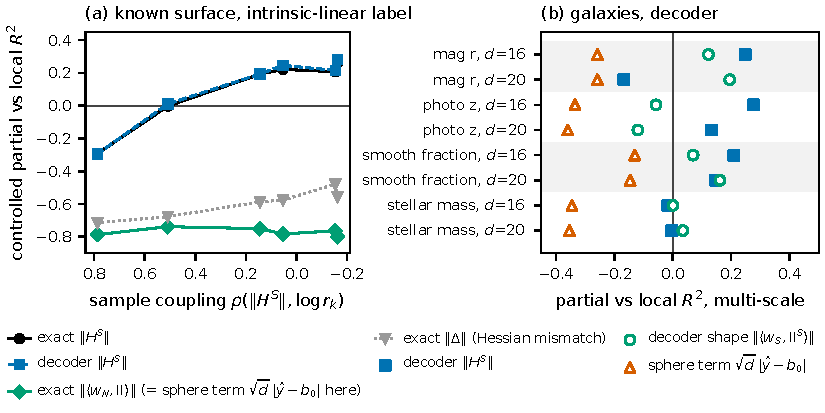
\includegraphics[width=0.85\textwidth]{figures/figF_mean_curvature.pdf}
\caption{(a) Known surface, linear label: partial against local $R^2$ as the density-curvature coupling is set by construction ($\gamma$ from $-1$ to $1$). (b) ViT-B galaxies: $\norm{\Htan}$ (filled squares), shape term (open circles), sphere term (open triangles). Figure from the workshop version.}
\label{fig:meancurv}
\end{figure}

\end{document}
